% ============================================================
%  MEMORIA DE PROYECTO — VISIÓN ARTIFICIAL
%  Sistema de Detección y Medición de Defectos en Baldosas
%  Cerámicas mediante Deep Learning (YOLOv8m-seg)
%
%  Compilar:
%    pdflatex memoria.tex && pdflatex memoria.tex
% ============================================================
\documentclass[12pt,a4paper]{article}

\usepackage[utf8]{inputenc}
\usepackage[T1]{fontenc}
\usepackage[spanish,es-tabla]{babel}
\usepackage{geometry}
\usepackage{graphicx}
\usepackage[hidelinks,colorlinks=true,linkcolor=blue!60!black,urlcolor=blue!60!black,citecolor=blue!60!black]{hyperref}
\usepackage{listings}
\usepackage{booktabs}
\usepackage{amsmath}
\usepackage{amssymb}
\usepackage{float}
\usepackage{xcolor}
\usepackage{fancyhdr}
\usepackage{titlesec}
\usepackage{enumitem}
\usepackage{multirow}
\usepackage{array}
\usepackage[protrusion=true,expansion=false]{microtype}
\usepackage{caption}
\usepackage{subcaption}
\usepackage{tocloft}
\usepackage{mdframed}
\usepackage{tabularx}

\geometry{a4paper, top=2.5cm, bottom=2.5cm, left=3cm, right=3cm}
\graphicspath{{imagenes/}}

\pagestyle{fancy}
\fancyhf{}
\fancyhead[L]{\small\textit{Detección de Defectos en Baldosas Cerámicas — YOLOv8m-seg}}
\fancyhead[R]{\small\thepage}
\fancyfoot[C]{\small Sistemas de Percepción y Visión Artificial · 3.º Ingeniería en la Industria Conectada}
\renewcommand{\headrulewidth}{0.4pt}
\renewcommand{\footrulewidth}{0.4pt}

\definecolor{codebg}{RGB}{30,40,55}
\definecolor{codegreen}{RGB}{106,180,95}
\definecolor{codeyellow}{RGB}{220,180,80}
\definecolor{codeblue}{RGB}{130,170,220}
\definecolor{codered}{RGB}{210,100,80}
\definecolor{codefg}{RGB}{212,228,250}
\definecolor{accent}{RGB}{255,182,144}

\lstdefinestyle{python}{
  language=Python,
  backgroundcolor=\color{codebg},
  basicstyle=\ttfamily\footnotesize\color{codefg},
  keywordstyle=\color{codeblue}\bfseries,
  stringstyle=\color{codegreen},
  commentstyle=\color{gray}\itshape,
  numberstyle=\tiny\color{gray},
  numbers=left, numbersep=8pt,
  breaklines=true, frame=single,
  rulecolor=\color{codebg!60!black},
  framesep=4pt, tabsize=4,
  showstringspaces=false, captionpos=b,
  morekeywords={True,False,None,as,from,import,yield,with},
  literate={á}{{\'a}}1 {é}{{\'e}}1 {í}{{\'i}}1 {ó}{{\'o}}1
           {ú}{{\'u}}1 {ñ}{{\~n}}1 {Á}{{\'A}}1 {É}{{\'E}}1
}
\lstset{style=python}

\titleformat{\section}{\Large\bfseries\color{accent!80!black}}{\thesection}{1em}{}[\titlerule]
\titleformat{\subsection}{\large\bfseries}{\thesubsection}{1em}{}
\titleformat{\subsubsection}{\normalsize\bfseries}{\thesubsubsection}{1em}{}

\newmdenv[linecolor=accent!70!black,backgroundcolor=accent!5!white,
  linewidth=1.2pt,frametitle={\small\bfseries Nota técnica},
  frametitlebackgroundcolor=accent!15!white]{technote}

% ============================================================
\begin{document}
\begin{titlepage}
  \centering
  \vspace*{1.5cm}
  {\LARGE\bfseries Sistemas de Percepción y Visión Artificial\par}
  \vspace{0.6cm}
  {\Large 3.º Grado en Ingeniería en la Industria Conectada\par}
  \vspace{2cm}
  \rule{\linewidth}{1.5pt}\\[0.4cm]
  {\huge\bfseries Sistema de Detección y Medición\\[0.3cm]
   de Defectos en Baldosas Cerámicas\\[0.3cm]
   mediante Deep Learning\par}
  \rule{\linewidth}{1.5pt}\\[1cm]
  {\large\textbf{Modelo:} YOLOv8m-seg · Segmentación de Instancias\par}
  \vspace{0.5cm}
  {\large\textbf{Pipeline:} Adquisición → Etiquetado → Pseudo-labeling\\
   → Entrenamiento → Inferencia → Aplicación Web\par}
  \vfill
  \begin{tabular}{rl}
    \textbf{Autor:}      & Javier Barba Berrocal \\[4pt]
    \textbf{Fecha:}      & \today \\[4pt]
    \textbf{Repositorio:} & \url{https://github.com/jaaviixoo06}\\
  \end{tabular}
  \vspace{1.5cm}
\end{titlepage}

% ── Resumen ───────────────────────────────────────────────────
\begin{abstract}
\noindent
El presente trabajo documenta el desarrollo íntegro de un sistema de visión artificial
orientado a la detección y cuantificación automática de defectos superficiales en
baldosas cerámicas industriales. La tipología de defectos contemplada abarca dos
categorías fundamentales: rayaduras —incisiones lineales o curvas sobre el esmalte—
y agujeros o desportillados —pérdidas puntuales de material—.

El pipeline construido comprende cinco fases integradas: adquisición y selección de
imágenes; preprocesado, etiquetado manual con Label Studio y etiquetado automático
por pseudo-labeling; entrenamiento de la red YOLOv8m-seg en GPU mediante la
plataforma Kaggle; un módulo de inferencia capaz de calcular la longitud, grosor y
área de cada defecto en milímetros reales; y una aplicación web interactiva construida
con FastAPI y HTML/JavaScript que permite inspeccionar cualquier imagen desde el
navegador y exportar el informe de resultados.

Los resultados sobre el conjunto de validación arrojan un Box\,mAP@0.5\,=\,0.806 y
Mask\,mAP@0.5\,=\,0.520, con tiempos de inferencia de aproximadamente 480\,ms en CPU.
El dataset final de entrenamiento consta de 2\,978 imágenes (2\,532 train + 446 val),
construido a partir de 148 anotaciones manuales ampliadas mediante pseudo-labeling
y aumentos con Albumentations.
\end{abstract}
\newpage

\tableofcontents
\newpage

% ============================================================
\section{Introducción y Motivación}
% ============================================================

La industria cerámica requiere un control de calidad exhaustivo de sus productos antes
de su comercialización. Es relevante señalar que las baldosas cerámicas pueden presentar
defectos generados tanto durante el proceso de fabricación como durante la manipulación
y el transporte: \textbf{rayaduras} —incisiones lineales o curvas que comprometen la
integridad superficial del esmalte— y \textbf{agujeros o desportillados} —pérdidas
localizadas de material que generan huecos de profundidad variable—.

La inspección visual humana, aun siendo el método tradicional, adolece de limitaciones
inherentes: es lenta, subjetiva y extraordinariamente propensa a la fatiga del operario.
En este contexto, la visión artificial emerge como la herramienta paradigmática para
automatizar este proceso con mayor repetibilidad, velocidad y trazabilidad. Resulta
imprescindible, por tanto, explorar las posibilidades que ofrece el aprendizaje profundo
aplicado a imágenes de dominio industrial específico.

\subsection{Objetivos del proyecto}

\begin{enumerate}[leftmargin=1.5cm]
  \item Construir un dataset propio de imágenes de baldosas cerámicas con defectos
        reales, anotadas a nivel de \emph{segmentación de instancias}.
  \item Entrenar un modelo de detección y segmentación (YOLOv8m-seg) capaz de
        localizar y contornear cada defecto con alta confianza.
  \item Implementar un módulo de medición que calcule la \textbf{longitud, grosor y
        área} de cada defecto en \textbf{milímetros reales} a partir de una única imagen.
  \item Desplegar el sistema en una \textbf{aplicación web} funcional, accesible
        desde cualquier navegador sin instalación de software adicional.
\end{enumerate}

\subsection{Clases de defecto}

Se han definido dos clases de defecto alineadas con la nomenclatura industrial. Cabe
mencionar que esta elección —aparentemente sencilla— es en sí misma el resultado de
una iteración experimental que se detalla en la Sección~\ref{sec:3clases}:

\begin{center}
\begin{tabular}{cll}
  \toprule
  \textbf{ID} & \textbf{Nombre} & \textbf{Descripción} \\
  \midrule
  0 & \texttt{agujero}  & Desportillado puntual; pérdida de material en el esmalte \\
  1 & \texttt{rayadura} & Incisión lineal o curva en la superficie de la baldosa \\
  \bottomrule
\end{tabular}
\end{center}

% ============================================================
\section{Fase 1 — Adquisición y Selección de Imágenes}
% ============================================================

\subsection{Contexto: fases de prueba PRUEBA1–PRUEBA5}

El proceso de adquisición de datos no fue lineal, sino progresivo e iterativo.
Lejos de partir de un conjunto de imágenes definitivo, se organizó el trabajo en
cinco fases de exploración —almacenadas bajo el directorio \texttt{testing/pruebas\_detector/}
del repositorio— que permitieron comprender el dominio visual del problema antes de
abordar el etiquetado a gran escala.

\begin{description}[leftmargin=2cm,style=nextline]
  \item[\texttt{PRUEBA1}]
    Primeras capturas fotográficas de baldosas del entorno del laboratorio.
    El objetivo no era aún construir un dataset, sino entender la variabilidad
    intrínseca del problema: resolución, iluminación, ángulo de captura y el grado
    de contraste de los defectos frente al esmalte.

  \item[\texttt{PRUEBA2}]
    Ampliación del número de muestras con la incorporación de baldosas que presentaban
    defectos de mayor envergadura. En esta fase se evaluó la calidad mínima de imagen
    requerida para que el etiquetado posterior fuera viable.

  \item[\texttt{PRUEBA3}]
    Primeras pruebas de anotación manual con herramientas básicas de dibujo de
    polígonos. Se detectaron dificultades específicas para anotar rayaduras finas
    de anchura inferior a $2\,$mm, cuyo contraste resulta insuficiente sin preprocesado.

  \item[\texttt{PRUEBA4}]
    Integración de Label Studio como plataforma de etiquetado profesional.
    En esta fase se definió el esquema de clases definitivo y se estableció el formato
    de exportación YOLO-seg como estándar del proyecto.

  \item[\texttt{PRUEBA5}]
    Fase de producción: directorio \texttt{base\_images} con \textbf{2\,690 imágenes}
    de alta calidad de baldosas cerámicas reales. Este directorio constituye la fuente
    principal tanto para el entrenamiento como para el pseudo-labeling posterior.
\end{description}

\subsection{Criterios de selección}

Para garantizar la calidad del dataset se establecieron los siguientes criterios de
admisión de imágenes, que actuaron como filtro previo al etiquetado:

\begin{itemize}
  \item La baldosa debe ocupar al menos el 60\,\% del encuadre de la imagen.
  \item Resolución mínima de $640\times 640$ píxeles.
  \item Iluminación uniforme, sin reflejos especulares que enmascaren los defectos.
  \item Presencia de al menos un defecto visible por imagen en el subconjunto de
        etiquetado manual.
\end{itemize}

\subsection{Datasets externos evaluados}

Asimismo, se evaluaron dos fuentes externas de datos como potenciales complementos
al dataset propio:

\begin{center}
\begin{tabularx}{\linewidth}{lXcc}
  \toprule
  \textbf{Dataset} & \textbf{Descripción} & \textbf{Imágenes} & \textbf{Adoptado} \\
  \midrule
  DATN Ceramic Tile & Baldosas cerámicas reales con defectos etiquetados & $\sim$800 & \textbf{Sí} \\
  DBCC Bridge Crack & Grietas en estructuras de hormigón y puentes & $\sim$32\,000 & No \\
  \bottomrule
\end{tabularx}
\end{center}

El dataset DBCC fue descartado a pesar de contener imágenes de grietas lineales
morfológicamente similares a las rayaduras. La razón determinante fue el \emph{domain
shift}: el dominio visual de una superficie gris rugosa de hormigón dista
considerablemente del esmalte cerámico liso y brillante, hasta el punto de que
entrenar con imágenes de hormigón introducía falsos positivos sistemáticos en
texturas de fondo de las baldosas. En consecuencia, se optó por privilegiar la
pureza del dominio sobre la cantidad bruta de datos.

% ============================================================
\section{Fase 2 — Tratamiento de Imágenes y Construcción del Dataset}
% ============================================================

\subsection{Evolución del aprendizaje en filtros: de las monedas a las baldosas}
\label{sec:filtros_evolucion}

Es relevante subrayar que el desarrollo del preprocesado de imágenes no partió
directamente de las baldosas cerámicas, sino de una progresión pedagógica que permitió
comprender el comportamiento de los filtros en contextos de creciente complejidad.
Esta metodología —de lo simple a lo complejo— resultó determinante para tomar
decisiones informadas sobre el preprocesado final del sistema.

\subsubsection{Primera etapa: detección de bordes sobre monedas}

El primer ejercicio de procesamiento de imagen se realizó sobre un conjunto de
\textbf{monedas de distintos tamaños y relieves}, que ofrecen un entorno controlado
para evaluar detectores de bordes clásicos: Canny, Sobel y Laplaciano.

\begin{figure}[H]
  \centering
  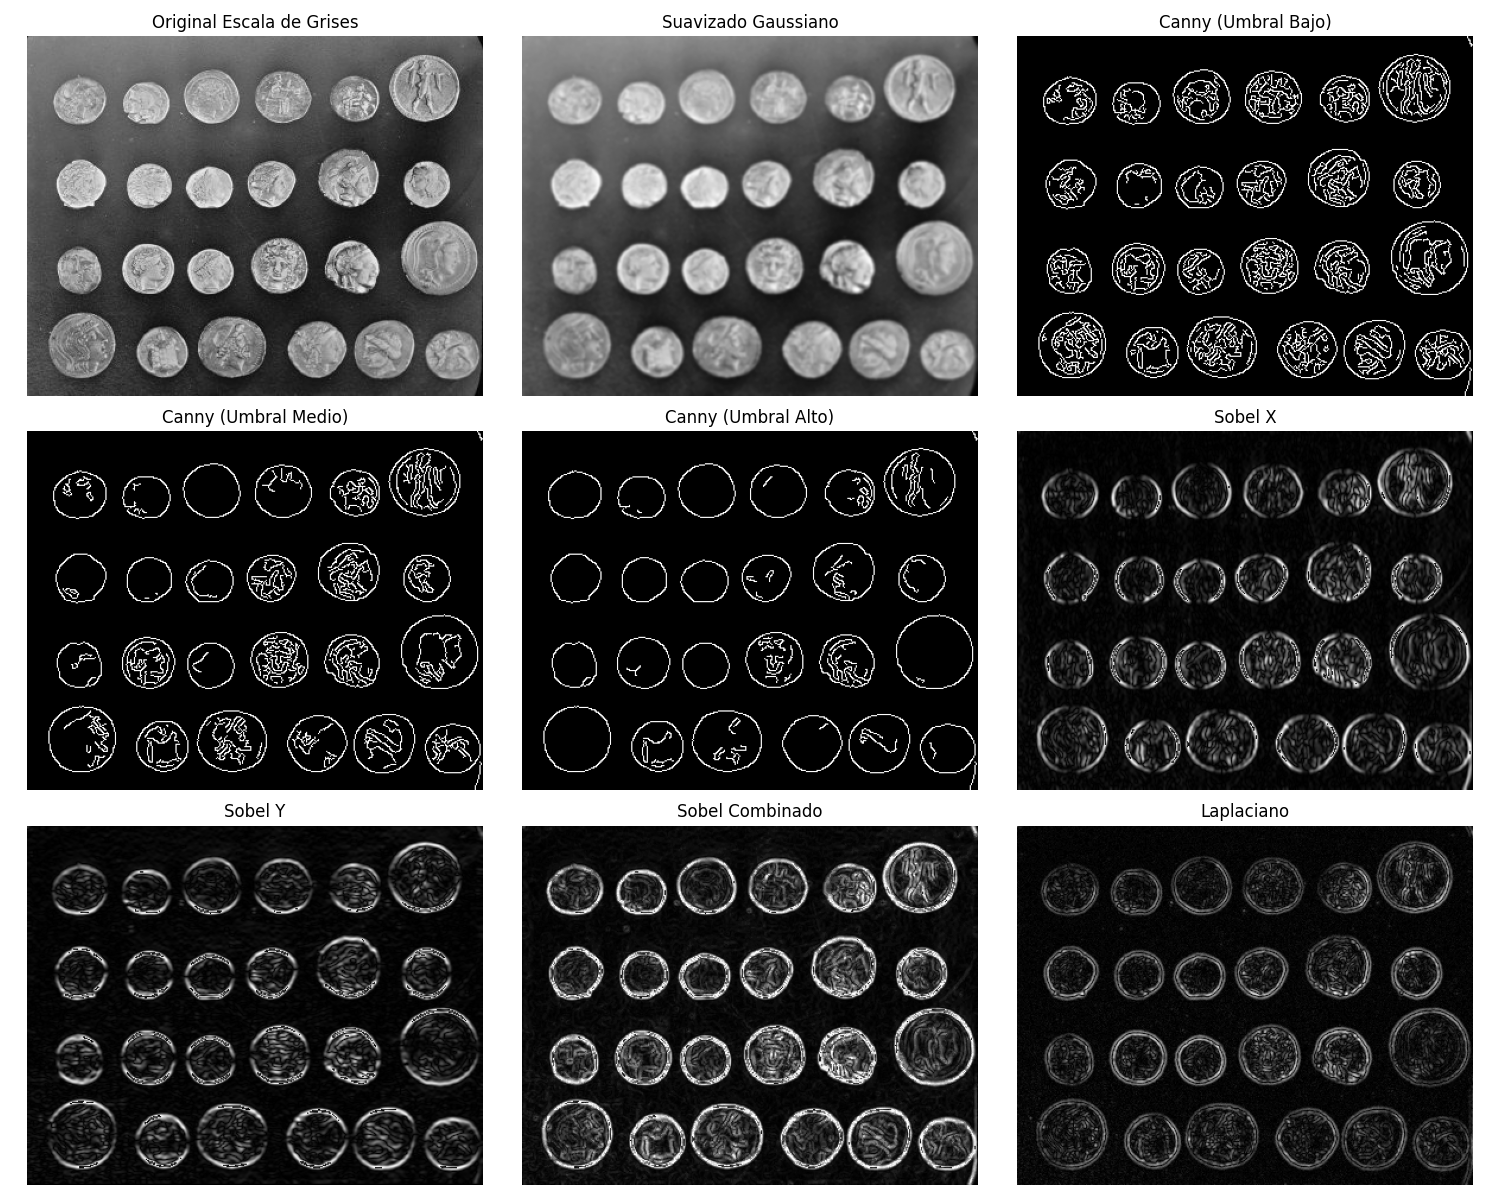
\includegraphics[width=0.90\linewidth]{deteccion_bordes}
  \caption{Comparativa de detectores de borde aplicados sobre monedas. De izquierda
    a derecha y de arriba a abajo: imagen original en escala de grises, suavizado
    gaussiano previo, Canny con umbral bajo (muchos bordes, ruido), Canny con umbral
    medio (equilibrado), Canny con umbral alto (solo bordes principales), Sobel en
    dirección X, Sobel en Y, Sobel combinado y Laplaciano. Esta comparativa permitió
    comprender la sensibilidad de cada operador frente al ruido y su capacidad de
    resaltar estructuras de diferente escala.}
  \label{fig:deteccion_bordes}
\end{figure}

\begin{figure}[H]
  \centering
  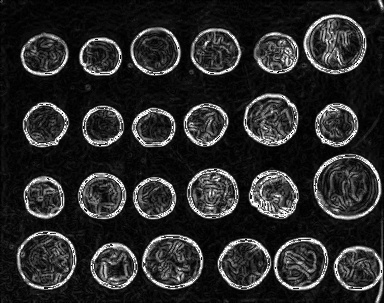
\includegraphics[width=0.65\linewidth]{sobel_combined}
  \caption{Resultado del filtro Sobel combinado ($\sqrt{G_x^2 + G_y^2}$) sobre el
    conjunto completo de monedas. La magnitud del gradiente resalta con claridad los
    contornos circulares y los relieves internos de cada moneda, aunque presenta
    mayor sensibilidad al ruido superficial que el operador Canny con umbral medio.}
  \label{fig:sobel_combined}
\end{figure}

De este ejercicio se extrajeron conclusiones fundamentales: el operador Canny con
umbral medio ofrece el mejor compromiso entre sensibilidad y robustez frente al ruido;
el Laplaciano, en cambio, amplifica el ruido de sensor de forma inaceptable en imágenes
de bajo contraste. No obstante, en el contexto de las baldosas cerámicas —cuyas rayaduras
presentan un perfil de contraste radicalmente diferente al de los relieves de una moneda—,
estos operadores de segundo orden demostraron ser insuficientes por sí solos.

\subsubsection{Segunda etapa: inpainting y Difference of Gaussians sobre imagen de carretera}

El segundo ejercicio abordó una problemática de mayor complejidad: la detección de
marcas viales sobre una \textbf{imagen de carretera nocturna}. En este caso, la
dificultad no residía en la detección de bordes, sino en la eliminación del ruido de
fondo (la textura del asfalto) para aislar únicamente las marcas de interés.

\begin{figure}[H]
  \centering
  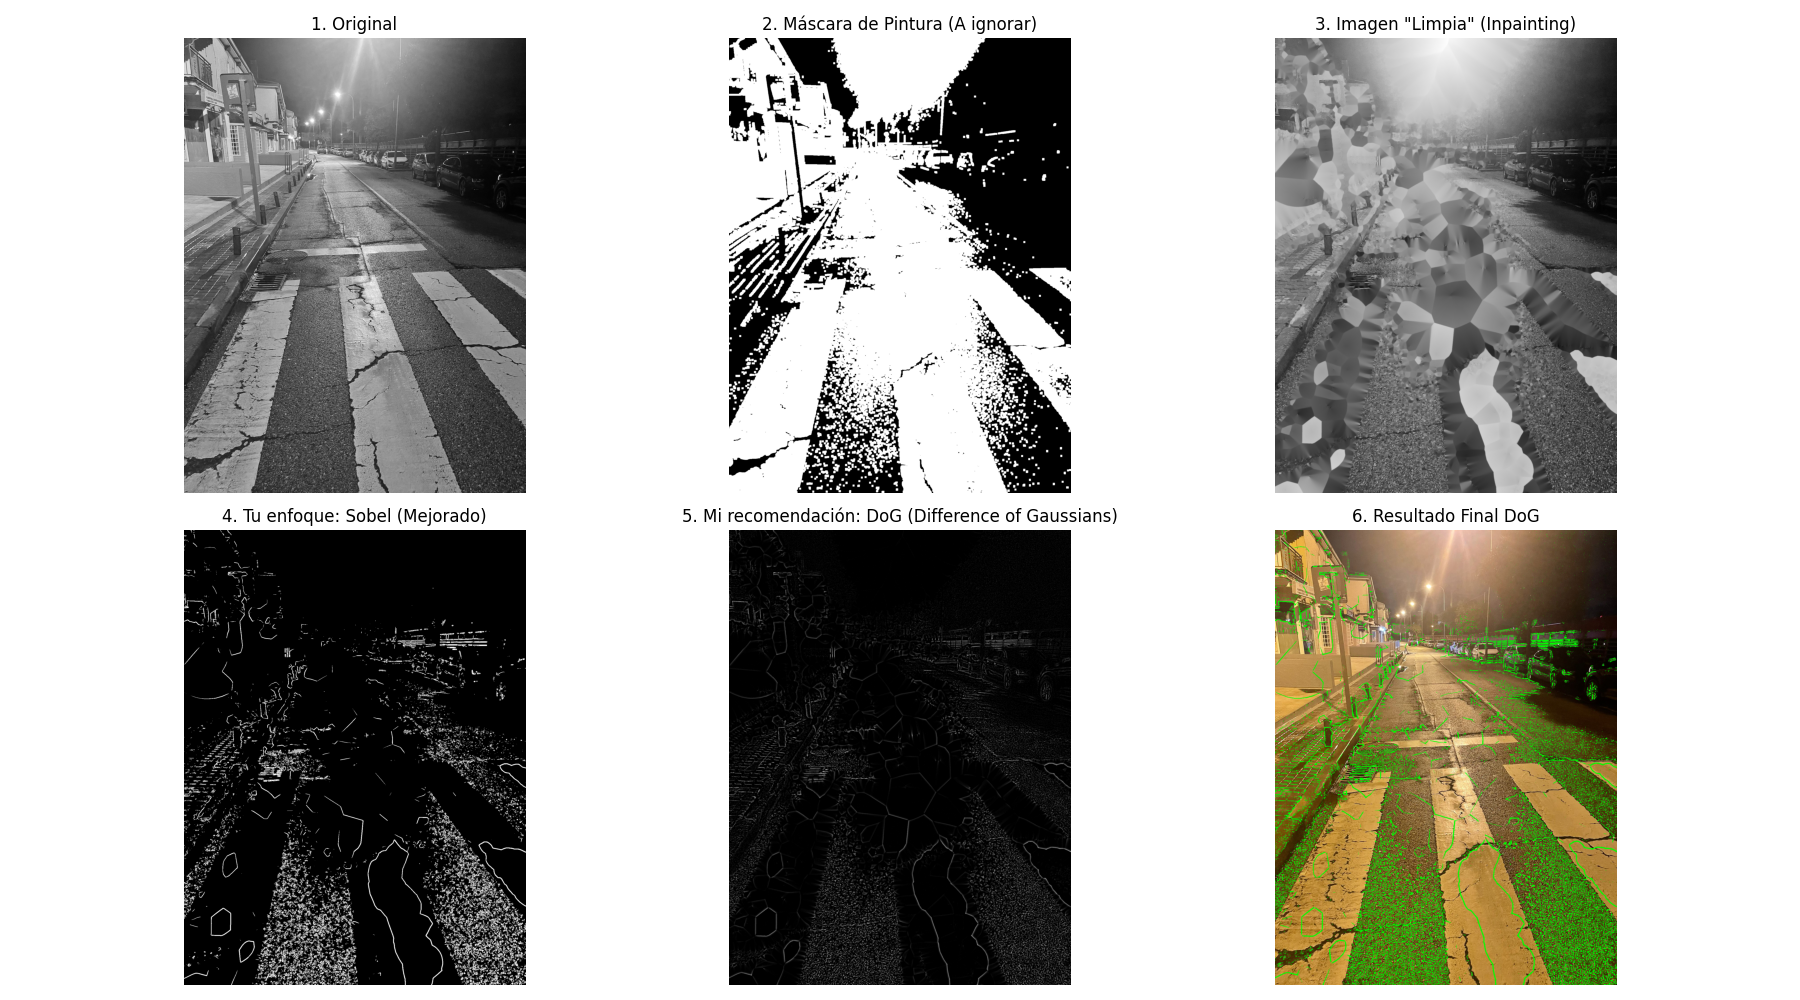
\includegraphics[width=0.90\linewidth]{comparativa_sobel_dog}
  \caption{Comparativa de dos estrategias sobre imagen de carretera. Arriba: imagen
    original, máscara de pintura (zonas a ignorar) e imagen limpia obtenida mediante
    \emph{inpainting}. Abajo: el enfoque inicial con Sobel (mejorado), la propuesta
    final con \emph{Difference of Gaussians} (DoG) y el resultado final. El DoG
    suprime el ruido de baja frecuencia de la textura del asfalto mientras preserva
    las estructuras finas de las marcas, demostrando ser significativamente superior
    al operador Sobel para este tipo de problema.}
  \label{fig:carretera_dog}
\end{figure}

El operador \textbf{Difference of Gaussians} (DoG) —diferencia entre dos imágenes
suavizadas con kernels gaussianos de distinto sigma— actúa como un filtro paso-banda
espacial: elimina tanto las frecuencias muy bajas (fondo uniforme) como las muy altas
(ruido de sensor), preservando las estructuras de tamaño intermedio. Este principio,
aprendido en el ejercicio de la carretera, resultó clave para orientar la elección del
filtro \emph{blackhat} morfológico en la aplicación final sobre baldosas.

\subsubsection{Tercera etapa: pipeline completo sobre baldosas cerámicas}

La aplicación directa de los aprendizajes anteriores al dominio objetivo condujo al
diseño de un pipeline de preprocesado específico para la detección de rayaduras en
baldosas. En este caso, la característica diferencial de las rayaduras —estructuras
oscuras y alargadas sobre un fondo claro y uniforme— hacía que el operador
\textbf{blackhat morfológico} fuera la herramienta más adecuada.

\begin{figure}[H]
  \centering
  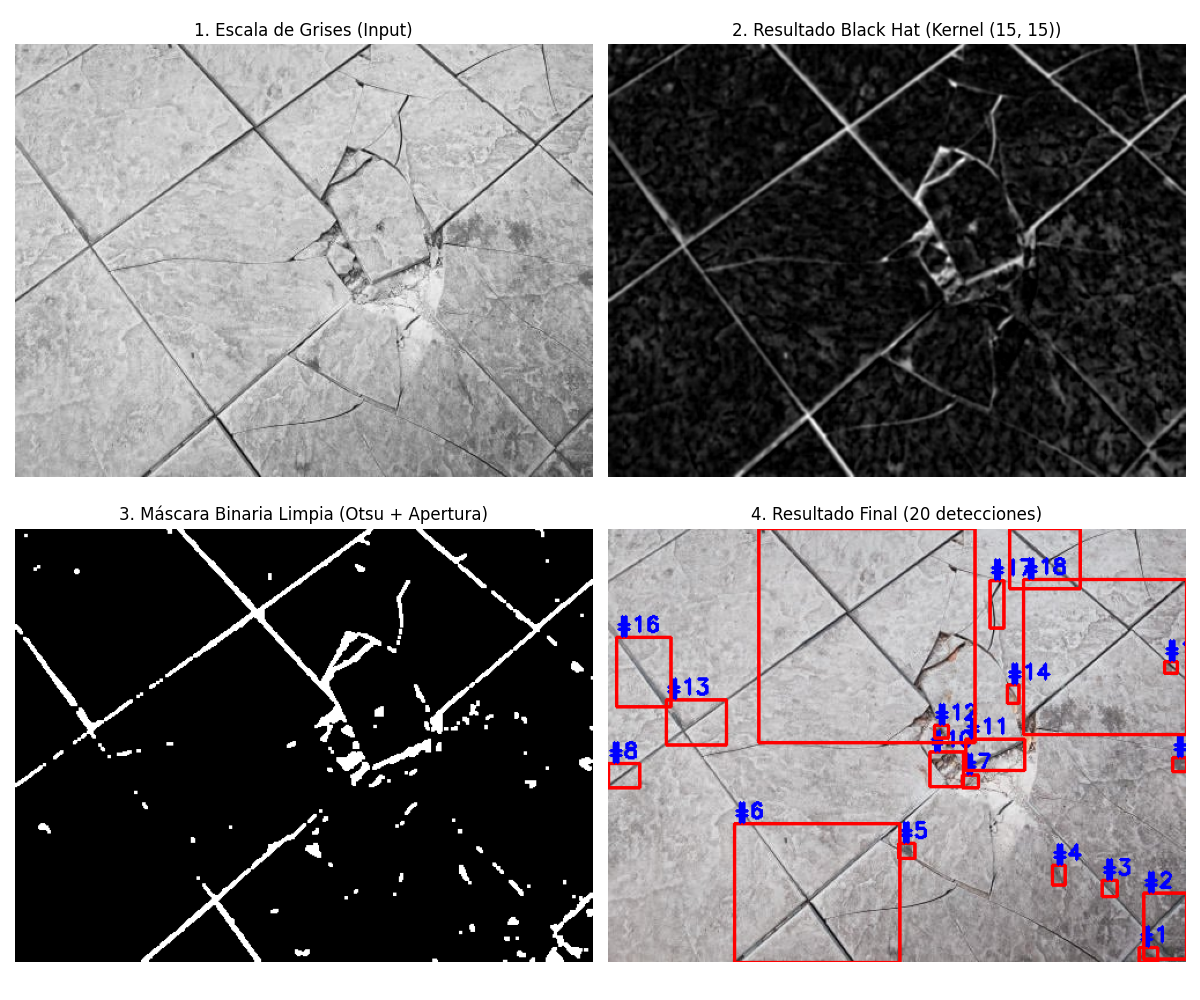
\includegraphics[width=0.88\linewidth]{resultado_deteccion_baldosas}
  \caption{Pipeline de preprocesado y detección sobre imagen de baldosa. (1) Imagen
    original en escala de grises; (2) resultado del filtro Black Hat con kernel
    $15\times 15$, que realza las rayaduras y juntas como estructuras oscuras sobre
    fondo claro; (3) máscara binaria obtenida tras umbralización de Otsu y operación
    morfológica de apertura, que elimina el ruido residual; (4) resultado final con
    20 detecciones etiquetadas. Este pipeline sirvió como referencia para el diseño
    de la segunda pasada de verificación en el módulo de inferencia.}
  \label{fig:pipeline_baldosas}
\end{figure}

\subsection{Filtros de preprocesado evaluados para el modelo}
\label{sec:filtros}

A la luz de la progresión anterior, se evaluaron cuatro técnicas de preprocesado
específicamente sobre el dataset de baldosas, con el objetivo de determinar cuáles
debían integrarse en el pipeline del modelo y cuáles debían descartarse.

\subsubsection{Umbralización binaria (Otsu)}

\begin{lstlisting}[caption={Umbralización de Otsu sobre canal de luminancia}]
gray = cv2.cvtColor(img, cv2.COLOR_BGR2GRAY)
_, thresh = cv2.threshold(gray, 0, 255,
                          cv2.THRESH_BINARY_INV + cv2.THRESH_OTSU)
\end{lstlisting}

La umbralización de Otsu calcula automáticamente el umbral óptimo minimizando la
varianza intraclase entre fondo y objeto. Aplicada sobre la baldosa —cuya superficie
es blanca y el fondo de la fotografía es oscuro—, el umbral resultante se sitúa
en torno a 60 y segmenta correctamente la baldosa del fondo. No obstante, no distingue
entre la superficie esmaltada y las rayaduras, cuyo contraste local es insuficiente
para esta operación global.

\textbf{Decisión}: adoptada exclusivamente para la calibración de escala px$\to$mm
en \texttt{detect\_tile\_px()}, no como preprocesado de entrada al modelo.

\subsubsection{Suavizado gaussiano}

\begin{lstlisting}[caption={Suavizado gaussiano con kernel 5$\times$5}]
blurred = cv2.GaussianBlur(img, (5, 5), sigmaX=1.5)
\end{lstlisting}

El suavizado gaussiano elimina ruido de sensor, pero atenúa simultáneamente los
bordes finos de las rayaduras. Para rayaduras de anchura inferior a $2\,$mm, el
suavizado llega a hacerlas prácticamente invisibles en el espacio de 640 píxeles.
Las pruebas empíricas con el modelo evidenciaron una pérdida de $\approx 1{-}2$ puntos
de mAP en validación respecto a la imagen original sin filtro.

\textbf{Decisión}: descartado como preprocesado global; se mantiene como paso
intermedio interno dentro de \texttt{detect\_tile\_px()} para reducir microestructuras
del esmalte que interferirían con la detección del contorno de la baldosa.

\subsubsection{CLAHE}

\begin{lstlisting}[caption={CLAHE en canal L del espacio de color LAB}]
lab = cv2.cvtColor(img, cv2.COLOR_BGR2LAB)
L, A, B = cv2.split(lab)
clahe = cv2.createCLAHE(clipLimit=2.0, tileGridSize=(8, 8))
L_eq  = clahe.apply(L)
img_clahe = cv2.cvtColor(cv2.merge([L_eq, A, B]), cv2.COLOR_LAB2BGR)
\end{lstlisting}

La ecualización adaptativa de histograma (CLAHE) opera sobre la luminancia en el
espacio LAB, mejorando el contraste local sin sobreexponer las zonas ya bien iluminadas.
En baldosas con gradientes de iluminación, resalta las rayaduras en las zonas de menor
exposición. Sin embargo, en condiciones de iluminación uniforme —predominantes en el
dataset— el efecto es mínimo o introduce artefactos de halo en los bordes de la baldosa.

\textbf{Decisión}: incluido como transformación de aumentación en Albumentations con
probabilidad 0.30, de modo que el modelo aprenda a generalizar ante variaciones de
contraste, pero no aplicado de forma fija en inferencia.

\subsubsection{Blackhat morfológico}

\begin{lstlisting}[caption={Filtro blackhat para realzar rayaduras oscuras sobre fondo claro}]
kernel   = cv2.getStructuringElement(cv2.MORPH_RECT, (15, 15))
blackhat = cv2.morphologyEx(gray, cv2.MORPH_BLACKHAT, kernel)
enhanced = cv2.addWeighted(gray, 1.0, blackhat, 2.5, 0)
\end{lstlisting}

El operador blackhat extrae las regiones más oscuras que su entorno local en un radio
definido por el kernel. En el caso de las baldosas —esmalte blanco con rayaduras como
incisiones oscuras—, con un kernel de $15\times 15$ y un factor de amplificación de
2.5 las rayaduras finas ganan entre 20 y 40 niveles de gris adicionales, haciéndolas
visualmente inequívocas incluso en zonas de bajo contraste.

\textbf{Decisión}: integrado en \texttt{src/infer.py} como canal auxiliar de
verificación. Cuando el modelo no detecta ningún defecto, se aplica blackhat como
segunda pasada para confirmar que no existen rayaduras de contraste extremadamente bajo.

\begin{figure}[H]
  \centering
  \begin{subfigure}[b]{0.30\linewidth}
    
\includegraphics[width=\linewidth]{filtro_original}
    \caption{Original}
  \end{subfigure}\hfill
  \begin{subfigure}[b]{0.30\linewidth}
    
\includegraphics[width=\linewidth]{filtro_clahe}
    \caption{CLAHE (clipLimit\,=\,2)}
  \end{subfigure}\hfill
  \begin{subfigure}[b]{0.30\linewidth}
    
\includegraphics[width=\linewidth]{filtro_blackhat}
    \caption{Blackhat $15\times 15$}
  \end{subfigure}
  \caption{Comparativa de los tres filtros evaluados sobre un recorte de
    $256\times 256\,$px extraído de una imagen de baldosa real. CLAHE mejora el
    contraste global de forma apreciable, pero el operador blackhat es el único que
    hace la rayadura claramente distinguible del fondo, confirmando su idoneidad como
    canal auxiliar de detección.}
  \label{fig:filtros}
\end{figure}

\subsubsection{Resumen de decisiones de preprocesado}

\begin{center}
\begin{tabular}{lcccl}
  \toprule
  \textbf{Filtro} & \textbf{Rayaduras gruesas} & \textbf{Rayaduras finas} & \textbf{Agujeros} & \textbf{Integración} \\
  \midrule
  Sin filtro           & \textbf{Bueno} & Regular  & \textbf{Bueno} & Entrada principal al modelo \\
  Threshold Otsu       & Regular  & Malo     & Regular  & Solo calibración de escala \\
  Gaussiano $5\times5$ & Regular  & Malo     & Regular  & Descartado \\
  CLAHE                & Bueno    & Regular  & Bueno    & Augmentación (prob.\,0.30) \\
  \textbf{Blackhat}    & Regular  & \textbf{Bueno} & Malo & Segunda pasada post-inferencia \\
  \bottomrule
\end{tabular}
\end{center}

La conclusión principal de este análisis es que no existe un único filtro óptimo para
todas las condiciones de defecto e iluminación. La estrategia adoptada —imagen original
como entrada al modelo, blackhat como canal de verificación— resulta más robusta que
cualquier preprocesado fijo de aplicación universal.

\subsection{Herramienta de etiquetado: Label Studio}

Se utilizó \textbf{Label Studio} (v1.x, modo local) como plataforma de anotación,
seleccionada tras evaluar las principales alternativas disponibles. Esta herramienta
permite etiquetar polígonos de segmentación directamente sobre la imagen en el
navegador y exportar en múltiples formatos, entre ellos el formato YOLO-seg nativo.

La configuración empleada fue la siguiente:
\begin{itemize}
  \item Tipo de tarea: \emph{Image Segmentation} con polígonos de instancia.
  \item Clases: \texttt{agujero} (color verde) y \texttt{rayadura} (color naranja/rojo).
  \item Exportación: formato YOLO-seg (coordenadas normalizadas de polígono).
\end{itemize}

El proceso de etiquetado evolucionó a través de dos fases diferenciadas cuya
distinción resulta determinante para comprender la calidad final del dataset.

\medskip
\noindent\textbf{Primera fase — bounding boxes para ambas clases.}
Tanto las rayaduras como los agujeros se etiquetaron inicialmente con rectángulos
envolventes. Para los agujeros —formas compactas y redondeadas— este esquema resultó
suficientemente preciso. Sin embargo, para las rayaduras —trazos curvos y delgados de
anchura de uno a tres píxeles— la caja envolvente capturaba una proporción
desproporcionada de esmalte intacto, contaminando las máscaras y degradando la
capacidad discriminativa del modelo.

\begin{figure}[H]
  \centering
  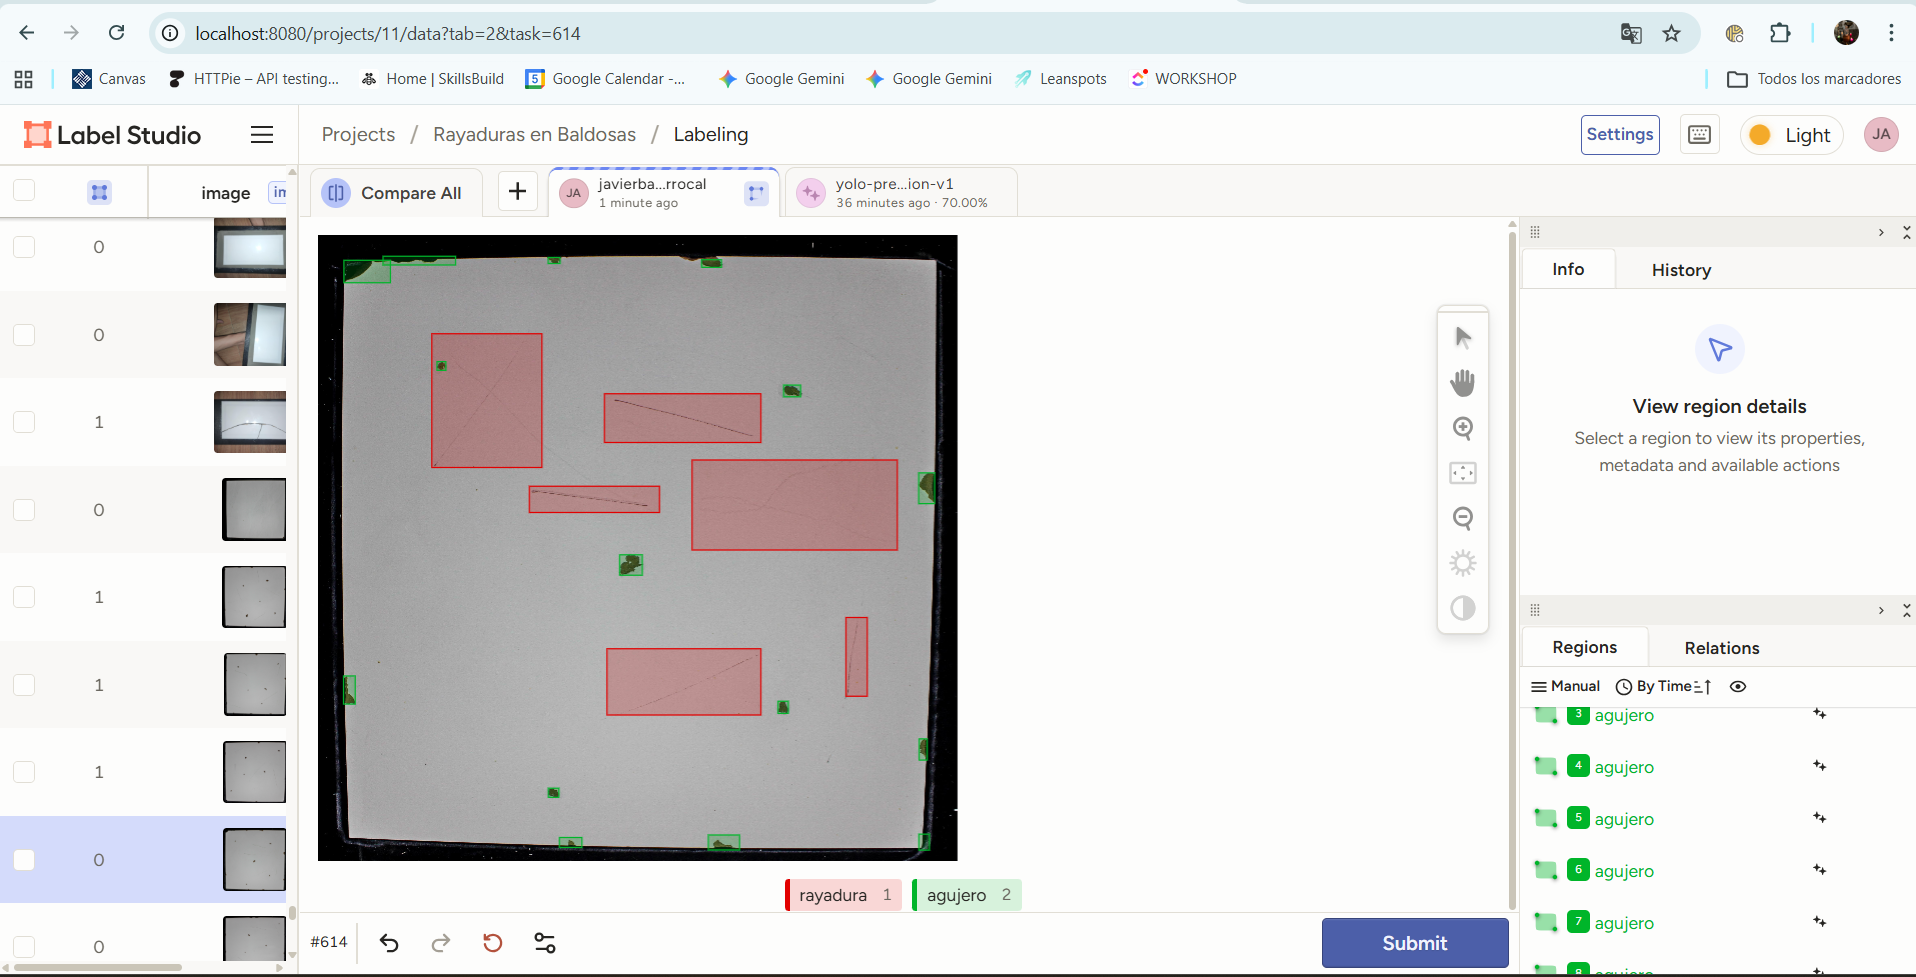
\includegraphics[width=0.90\linewidth]{label_studio_pseudo}
  \caption{Label Studio durante la \textbf{primera fase} de etiquetado: ambas clases
    —\texttt{rayadura} y \texttt{agujero}— se anotan con bounding boxes rectangulares.
    Los rectángulos rosas delimitan las regiones marcadas sobre la baldosa. Para los
    agujeros, de forma compacta, esta representación resultó válida; para las rayaduras,
    la caja envolvente incluía demasiado esmalte intacto, lo que degradaba la calidad
    de las máscaras de segmentación y motivó la transición al etiquetado poligonal.}
  \label{fig:pseudo_ls}
\end{figure}

\medskip
\noindent\textbf{Segunda fase — polígonos de precisión para rayaduras.}
Reconocida esta limitación, se migró al etiquetado poligonal exclusivamente para la
clase \texttt{rayadura}, trazando el contorno real de cada incisión vértice a vértice.
Los agujeros mantuvieron la representación rectangular, suficiente para su forma
compacta. Esta decisión elevó el coste de anotación por imagen pero se tradujo en una
ganancia sustancial en la precisión de las máscaras y, por extensión, en la calidad de
las mediciones métricas calculadas en inferencia.

El proceso de etiquetado manual resultó en \textbf{148 imágenes} anotadas,
con un total estimado de 320 instancias de defecto entre ambas clases.

\begin{figure}[H]
  \centering
  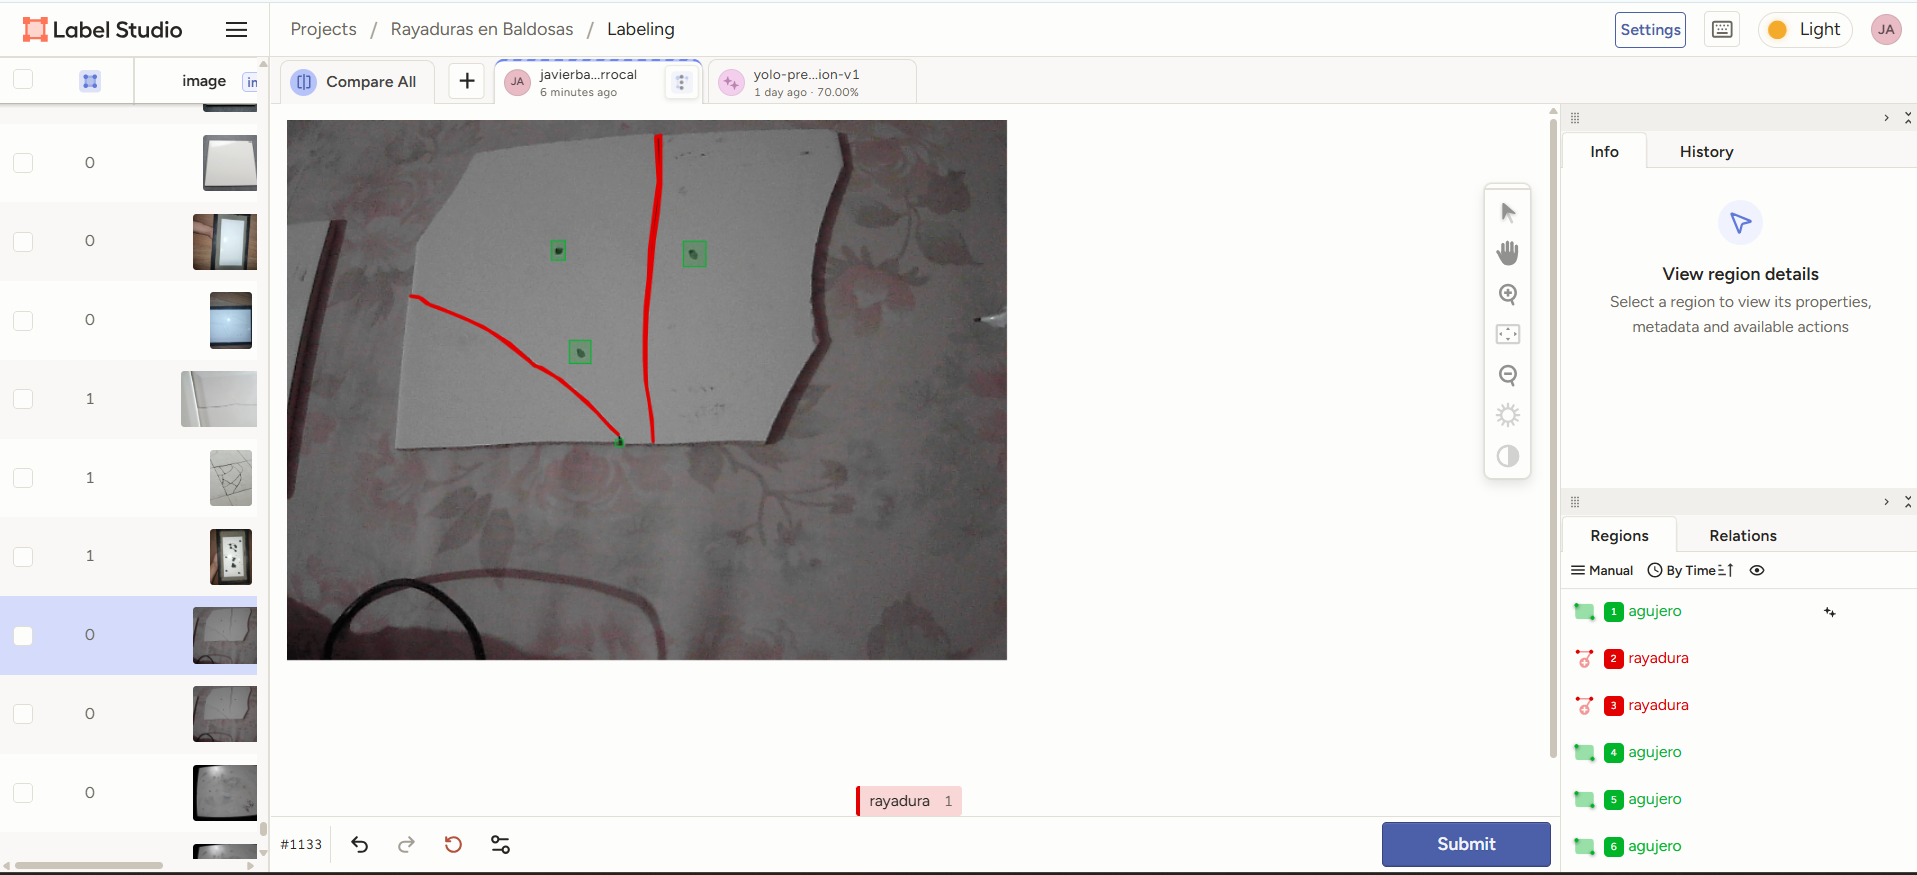
\includegraphics[width=0.90\linewidth]{label_studio_anotacion}
  \caption{Label Studio durante la \textbf{segunda fase} de etiquetado: las rayaduras
    se anotan con polígonos de precisión vértice a vértice. Los trazos rojos ciñen
    exactamente cada incisión sobre la superficie esmaltada, frente al esquema de
    bounding boxes de la primera fase. El panel lateral derecho lista las regiones bajo
    la clase \texttt{rayadura}; el proyecto se ejecutó en modo local sobre
    \texttt{localhost:8080}. La anotación poligonal proporciona la información de contorno
    necesaria para calcular dimensiones métricas reales en inferencia, algo imposible
    con simples rectángulos envolventes.}
  \label{fig:label_studio}
\end{figure}

\begin{figure}[H]
  \centering
  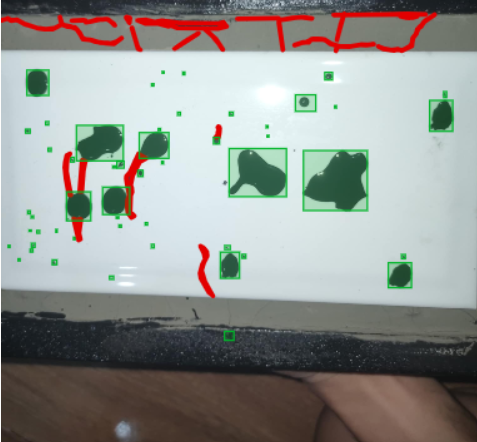
\includegraphics[width=0.80\linewidth]{prueba_deteccion}
  \caption{Resultado de inferencia sobre una baldosa real tras la segunda fase de
    etiquetado. Las máscaras rojas ciñen con precisión cada rayadura y los contornos
    verdes delimitan con exactitud los agujeros y desportillados. El salto cualitativo
    respecto a la primera fase —en la que los bounding boxes incluían fondo— es
    apreciable en la nitidez de los contornos de segmentación.}
  \label{fig:prueba_deteccion}
\end{figure}

\subsubsection*{Justificación de la elección de Label Studio}

\begin{center}
\begin{tabular}{llcc}
  \toprule
  \textbf{Herramienta} & \textbf{Tipo de anotación} & \textbf{Export YOLO-seg} & \textbf{Gratuita} \\
  \midrule
  Roboflow       & Polígono, caja, keypoint & Sí (con cuenta)  & Parcial \\
  CVAT           & Polígono completo        & Sí (convertido)  & \textbf{Sí} \\
  \textbf{Label Studio} & \textbf{Polígono completo} & \textbf{Sí nativo} & \textbf{Sí} \\
  \bottomrule
\end{tabular}
\end{center}

Label Studio fue elegido por su exportación directa al formato YOLO-seg sin conversión
intermedia, su instalación local sin límite de imágenes y su capacidad de usar el mismo
proyecto para comparar anotaciones manuales con predicciones del modelo en el flujo
de pseudo-labeling.

\subsection{Formato de etiquetas YOLO-seg}

Cada fichero de etiqueta (\texttt{.txt}) contiene una línea por instancia de defecto:
\begin{center}
\texttt{clase\ $x_1$\ $y_1$\ $x_2$\ $y_2$\ \ldots\ $x_n$\ $y_n$}
\end{center}
donde \texttt{clase} $\in \{0,1\}$ y las coordenadas están normalizadas respecto
al ancho y alto de la imagen ($\in [0,1]$). Este formato permite representar
contornos arbitrariamente complejos con la precisión requerida para la
segmentación de instancias.

\subsection{Pseudo-labeling: ampliación semi-supervisada del dataset}

Dado el elevado coste de la anotación manual —estimado en aproximadamente 8 minutos
por imagen para rayaduras complejas—, se implementó un pipeline de
\textbf{pseudo-labeling} que utiliza el propio modelo entrenado para generar etiquetas
sobre las imágenes no anotadas del dataset. Esta técnica, enmarcada en el ámbito del
aprendizaje semi-supervisado, permitió multiplicar el tamaño del dataset de forma
controlada y verificable.

\subsubsection{Algoritmo}

\begin{enumerate}
  \item Entrenar un modelo inicial $M_0$ con las 148 muestras manuales.
  \item Aplicar $M_0$ sobre las 2\,690 imágenes de \texttt{testing/pruebas\_detector/PRUEBA5/base\_images}.
  \item Aceptar únicamente las predicciones con confianza $\geq 0.65$.
  \item Combinar las etiquetas aceptadas con las manuales y reentrenar el modelo.
  \item Repetir con el modelo mejorado $M_1$ para obtener pseudo-etiquetas de mayor calidad.
\end{enumerate}

\begin{technote}
El umbral de 0.65 es crítico. Por debajo de este valor se aceptan falsos positivos en
exceso —el modelo confunde el fondo o las juntas con rayaduras—; por encima se descartan
detecciones válidas difíciles. El valor se determinó empíricamente observando 50
predicciones aleatorias a distintos umbrales.
\end{technote}

\begin{lstlisting}[caption={Núcleo del algoritmo de pseudo-labeling (\texttt{scripts/pseudo\_label.py})}]
def pseudo_label_images(image_paths, conf_thresh):
    model = YOLO("outputs/runs/scratch_yolo/weights/best.pt")
    pairs = []
    for img_path in image_paths:
        if cv2.imread(str(img_path)) is None:
            continue
        try:
            results = model.predict(
                str(img_path), conf=conf_thresh,
                iou=0.45, imgsz=640, verbose=False
            )
        except Exception:
            continue
        r = results[0]
        if r.boxes is None or len(r.boxes) == 0:
            continue
        labels = []
        for j, box in enumerate(r.boxes):
            cls_id = int(box.cls[0])
            has_mask = r.masks is not None and cls_id == 1
            if has_mask:
                poly = r.masks.xy[j]
                coords = [(float(px)/img_w, float(py)/img_h)
                          for px, py in poly]
                if len(coords) >= 3:
                    labels.append((cls_id, coords))
            else:
                x1,y1,x2,y2 = box.xyxy[0].tolist()
                labels.append((cls_id, [
                    (x1/img_w, y1/img_h), (x2/img_w, y1/img_h),
                    (x2/img_w, y2/img_h), (x1/img_w, y2/img_h)]))
        if labels:
            pairs.append((img_path, labels))
    return pairs
\end{lstlisting}

\subsubsection{Resultados por ronda}

\begin{center}
\begin{tabular}{lrrrr}
  \toprule
  \textbf{Ronda} & \textbf{Modelo base} & \textbf{Candidatas} & \textbf{Aceptadas} & \textbf{Tasa acept.} \\
  \midrule
  1 & \texttt{best.pt}  & 2\,690 & 1\,118 & 41,6\,\% \\
  2 & \texttt{best4.pt} & 2\,690 & 1\,014 & 37,7\,\% \\
  \bottomrule
\end{tabular}
\end{center}

La segunda ronda produjo menos pseudo-etiquetas pero de mayor calidad: el modelo más
maduro es más restrictivo en la asignación de confianza alta, lo que se traduce en una
precisión superior de las etiquetas aceptadas y un menor número de correcciones manuales
necesarias.

\subsection{Aumento de datos}

Cada par imagen–etiqueta fue aumentado $\times 4$ mediante la librería
\textbf{Albumentations}, preservando la coherencia geométrica de los polígonos
mediante el mecanismo \texttt{KeypointParams}:

\begin{center}
\begin{tabular}{llr}
  \toprule
  \textbf{Transformación} & \textbf{Descripción} & \textbf{Prob.} \\
  \midrule
  \texttt{HorizontalFlip}          & Espejo horizontal                             & 0.50 \\
  \texttt{VerticalFlip}            & Espejo vertical                               & 0.30 \\
  \texttt{RandomRotate90}          & Rotación en múltiplos de 90°                  & 0.40 \\
  \texttt{ShiftScaleRotate}        & Traslación $\pm 5\%$, escala $\pm 10\%$, rot. $\pm 20°$ & 0.60 \\
  \texttt{RandomBrightnessContrast}& Brillo $\pm 35\%$, contraste $\pm 35\%$      & 0.70 \\
  \texttt{HueSaturationValue}      & Tono $\pm 10$, sat. $\pm 25$, val $\pm 25$   & 0.50 \\
  \texttt{CLAHE}                   & Ecualización local adaptativa de histograma   & 0.30 \\
  \bottomrule
\end{tabular}
\end{center}

Asimismo, todas las imágenes se normalizaron a $640\times 640$ píxeles mediante
\textbf{letterboxing}: escala con preservación de relación de aspecto y relleno con
valor $114$ (gris neutro por defecto en YOLOv8). Cambiar este valor a 0 en pruebas
produjo una caída de $\approx 0.5$ puntos de mAP, lo que confirma la relevancia de
este parámetro aparentemente menor.

\subsection{Composición final del dataset}

\begin{center}
\begin{tabular}{lrr}
  \toprule
  \textbf{Origen} & \textbf{Imágenes originales} & \textbf{Tras aug. ×4} \\
  \midrule
  Etiquetado manual        & 148    & $\approx 592$   \\
  Pseudo-labeling (ronda 2)& 1\,014 & $\approx 4\,056$ \\
  \midrule
  \textbf{Total sin split} & \textbf{1\,162} & \textbf{2\,978} \\
  \midrule
  Train (85\,\%)           & —      & 2\,532 \\
  Val   (15\,\%)           & —      &   446 \\
  \bottomrule
\end{tabular}
\end{center}

% ============================================================
\section{Fase 3 — Entrenamiento del Modelo}
% ============================================================

\subsection{La decisión de consolidar clases: del fracaso de tres a la solidez de dos}
\label{sec:3clases}

En primera instancia, el modelo se entrenó con \textbf{tres subcategorías} diferenciadas
por el tamaño de la rayadura: \texttt{Rayadura\_Grande}, \texttt{Rayadura\_Normal} y
\texttt{Rayadura\_Pequeña}. La intuición subyacente era que una clasificación más granular
permitiría priorizar la reparación de los defectos más severos en un contexto industrial.
Los resultados, sin embargo, fueron inequívocos en su negativa.

\begin{figure}[H]
  \centering
  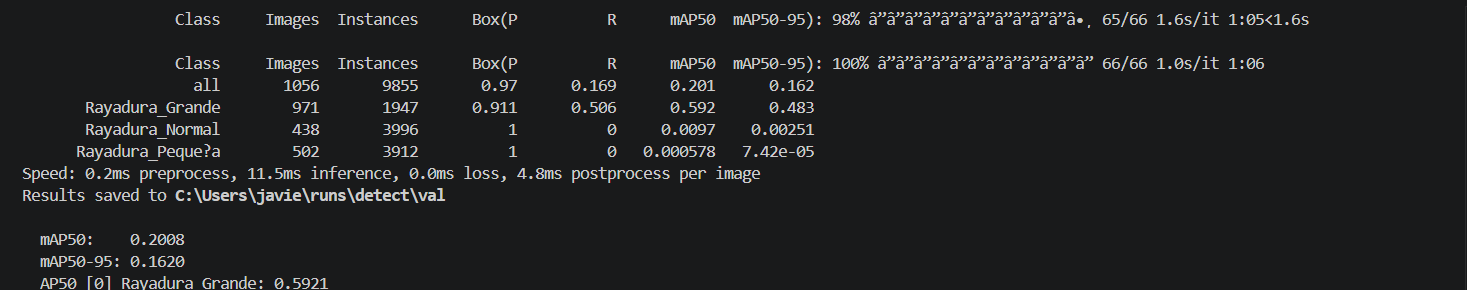
\includegraphics[width=0.90\linewidth]{early_model_metricas}
  \caption{Métricas de validación del primer modelo entrenado con tres subcategorías
    de rayadura. Solo \texttt{Rayadura\_Grande} alcanza un mAP50 aceptable (0.592)
    con Box(P)\,=\,0.911; \texttt{Rayadura\_Normal} (mAP50\,=\,0.0097) y
    \texttt{Rayadura\_Pequeña} (mAP50\,=\,0.000578) son estadísticamente nulas.
    La media global de mAP50\,=\,0.2008 hizo evidente que la granularidad de tres
    clases era inviable con el dataset disponible.}
  \label{fig:early_model}
\end{figure}

\begin{center}
\begin{tabular}{lcc}
  \toprule
  \textbf{Clase} & \textbf{mAP@0.50} & \textbf{Interpretación} \\
  \midrule
  Rayadura\_Grande  & 0.592 & Aprendida correctamente \\
  Rayadura\_Normal  & $\approx 0.010$ & Modelo incapaz de distinguirla \\
  Rayadura\_Pequeña & $\approx 0.001$ & Completamente ignorada \\
  \midrule
  \textbf{Media}    & \textbf{0.2008} & — \\
  \bottomrule
\end{tabular}
\end{center}

El análisis del fallo identificó tres causas concurrentes. En primer lugar, la
\textbf{ambigüedad intrínseca de la etiqueta}: la frontera entre «grande», «normal»
y «pequeña» es subjetiva, y dos anotadores distintos clasificarían la misma rayadura de
forma diferente, introduciendo ruido sistemático en las etiquetas. En segundo lugar, el
\textbf{desequilibrio de clases}: la mayoría de los ejemplos etiquetados correspondían
a \texttt{Rayadura\_Grande} por ser más fáciles de identificar visualmente. Por último,
la \textbf{similitud de representación visual}: en el espacio de $640\times 640\,$px,
las diferencias de tamaño entre categorías son de pocos píxeles, sin información
espacial suficiente para discriminarlas.

En consecuencia, se optó por consolidar las tres subcategorías en una única clase
\texttt{rayadura}. Esta decisión fue \textbf{óptima por tres razones}: eliminó la
ambigüedad de etiquetado, triplicó el número efectivo de ejemplos por clase, y transfirió
el cálculo del tamaño del defecto a la fase de inferencia —mediante \texttt{cv2.minAreaRect}—,
donde se puede calcular con precisión milimétrica sin necesidad de clasificarlo
durante el entrenamiento. El salto de mAP50 tras la consolidación fue de
$0.20 \to 0.74$ (piloto YOLOv8s-seg) y luego a $\mathbf{0.806}$ con el modelo final.

\subsection{Arquitectura: YOLOv8m-seg}

Se eligió la familia \textbf{YOLOv8} (Ultralytics, 2023) en su variante
\textbf{medium-segmentation} (\texttt{yolov8m-seg}), que combina detección de cajas
delimitadoras con segmentación de instancias a nivel de píxel. La elección de esta
arquitectura responde a una evaluación ponderada entre capacidad del modelo y
recursos disponibles:

\begin{center}
\begin{tabular}{lccc}
  \toprule
  \textbf{Variante} & \textbf{Parámetros} & \textbf{mAP50 COCO} & \textbf{Elegida} \\
  \midrule
  YOLOv8n-seg &  3,4\,M &  36,7 & No — insuficiente para dominio específico \\
  YOLOv8s-seg & 11,8\,M &  44,6 & Solo piloto inicial \\
  \textbf{YOLOv8m-seg} & \textbf{27,3\,M} & \textbf{51,0} & \textbf{Sí — equilibrio óptimo} \\
  YOLOv8l-seg & 46,0\,M &  52,4 & No — VRAM insuficiente con batch\,=\,8 \\
  YOLOv8x-seg & 71,8\,M &  53,4 & No — VRAM insuficiente \\
  \bottomrule
\end{tabular}
\end{center}

La versión \emph{small} se empleó en las primeras rondas de entrenamiento como piloto
y se migró a \emph{medium} para la ronda de producción, mejorando el mAP en
aproximadamente 6 puntos porcentuales. Las variantes \emph{large} y \emph{extra} fueron
descartadas porque la GPU T4 de Kaggle (16\,GB VRAM) alcanzaba el límite de memoria
con batch\,=\,8 para YOLOv8l.

La arquitectura de YOLOv8 sigue el paradigma \emph{anchor-free} y se articula en tres
componentes: \textbf{backbone} CSPDarknet con conexiones C2f; \textbf{neck} PANet para
fusión multi-escala en tres resoluciones ($P3, P4, P5$); y \textbf{head} con cabeza de
detección desacoplada más cabeza de segmentación basada en 32 prototipos de máscara.

\subsection{Historia de las plataformas de entrenamiento}
\label{sec:plataformas}

El proceso de entrenamiento atravesó tres plataformas distintas, cada una condicionada
por las limitaciones de la anterior. Esta evolución ilustra con claridad la importancia
crítica del hardware en proyectos de aprendizaje profundo.

\subsubsection{Primer intento: CPU local (Intel Core i7, 14 horas)}

El entrenamiento inicial se lanzó en el ordenador personal, equipado con un
\textbf{Intel Core i7} sin aceleración CUDA disponible. YOLOv8 puede ejecutarse en CPU,
pero el rendimiento es dramáticamente inferior:

\begin{center}
\begin{tabular}{ll}
  \toprule
  \textbf{Parámetro} & \textbf{Valor} \\
  \midrule
  Dispositivo         & CPU Intel Core i7 (8 núcleos, sin GPU CUDA) \\
  Batch size          & 4 (limitado por RAM) \\
  Épocas planificadas & 100 \\
  Tiempo por época    & $\approx$8,5 minutos \\
  Tiempo total        & $\approx$\textbf{14 horas} \\
  mAP50 final         & $\approx$0.58 \\
  \bottomrule
\end{tabular}
\end{center}

El tiempo de 14 horas es consecuencia directa de que cada \emph{forward pass} sobre
un batch de 4 imágenes tarda $\approx 2\,$s en CPU frente a $\approx 80\,$ms en GPU T4
—un factor de 25×—. Este resultado evidenció la inviabilidad del entrenamiento local
para iterar con rapidez y motivó la migración inmediata a recursos cloud con GPU.

\subsubsection{Segundo intento: Google Colab (interrumpido en la época 140/150)}

Como solución natural, el entrenamiento se migró a \textbf{Google Colab} con GPU T4
gratuita. El tiempo por época se redujo a $\approx 1,3$ minutos —tiempo total estimado
de $\approx 3,2$ horas para 150 épocas—. No obstante, surgió un contratiempo crítico:
la sesión fue \textbf{interrumpida automáticamente al alcanzar el límite de uso
gratuito}, cuando el entrenamiento llevaba $\approx 140$ de las 150 épocas planificadas.
Los pesos del modelo se perdieron al cerrarse la sesión sin completar el guardado.

Para mitigar este riesgo en futuras ejecuciones, se implementó un mecanismo de backup
automático mediante un hilo daemon que copiaba \texttt{last.pt} a Google Drive cada
600 segundos:

\begin{lstlisting}[caption={Mecanismo de backup automático en Google Colab}]
import threading, shutil, time, os

def _auto_backup(src_dir, dst_dir, interval=600):
    while True:
        time.sleep(interval)
        for fname in ("last.pt", "best.pt"):
            src = os.path.join(src_dir, fname)
            if os.path.exists(src):
                shutil.copy2(src, os.path.join(dst_dir, fname))
                print(f"[BACKUP] {fname} guardado en Drive")

t = threading.Thread(target=_auto_backup,
                     args=("/content/runs/scratch_yolo/weights",
                           "/content/drive/MyDrive/yolo_backup"))
t.daemon = True
t.start()
\end{lstlisting}

\subsubsection{Solución definitiva: Kaggle Notebooks (150 épocas en 3,2 horas)}

La interrupción de Colab motivó la migración definitiva a \textbf{Kaggle Notebooks}.
Las ventajas sobre Colab en el contexto específico de este proyecto son sustanciales:

\begin{center}
\begin{tabularx}{\linewidth}{lXX}
  \toprule
  \textbf{Aspecto} & \textbf{Google Colab (gratuito)} & \textbf{Kaggle (gratuito)} \\
  \midrule
  GPU disponible    & T4 (16\,GB)              & \textbf{T4 $\times$ 2 (32\,GB)} \\
  Tiempo/semana     & Variable, no garantizado & \textbf{30 h semanales garantizadas} \\
  Sesión máxima     & $\leq$12 h (90 min inactivo) & \textbf{$\leq$12 h continuas} \\
  Persistencia      & Manual vía Drive         & \textbf{Datasets y outputs nativos} \\
  \bottomrule
\end{tabularx}
\end{center}

El entrenamiento completo de \textbf{150 épocas se completó en 3,2 horas} con
batch\,=\,8, imgsz\,=\,640. Los pesos finales se descargaron como artefacto del
notebook, almacenándose en \texttt{outputs/runs/scratch\_yolo/weights/best5.pt}.

\subsection{Hiperparámetros de entrenamiento}

\begin{center}
\begin{tabular}{ll}
  \toprule
  \textbf{Parámetro} & \textbf{Valor} \\
  \midrule
  \texttt{epochs}         & 150    \\
  \texttt{imgsz}          & 640    \\
  \texttt{batch}          & 8      \\
  \texttt{patience}       & 30     \\
  \texttt{lr0}            & 0.01   \\
  \texttt{lrf}            & 0.01   \\
  \texttt{momentum}       & 0.937  \\
  \texttt{weight\_decay}  & 0.0005 \\
  \texttt{warmup\_epochs} & 3      \\
  \texttt{mosaic}         & 1.0    \\
  \texttt{mixup}          & 0.1    \\
  \texttt{box}            & 7.5    \\
  \texttt{cls}            & 1.5    \\
  \texttt{dfl}            & 1.5    \\
  \bottomrule
\end{tabular}
\end{center}

\subsection{Progresión del entrenamiento}

\begin{figure}[H]
  \centering
  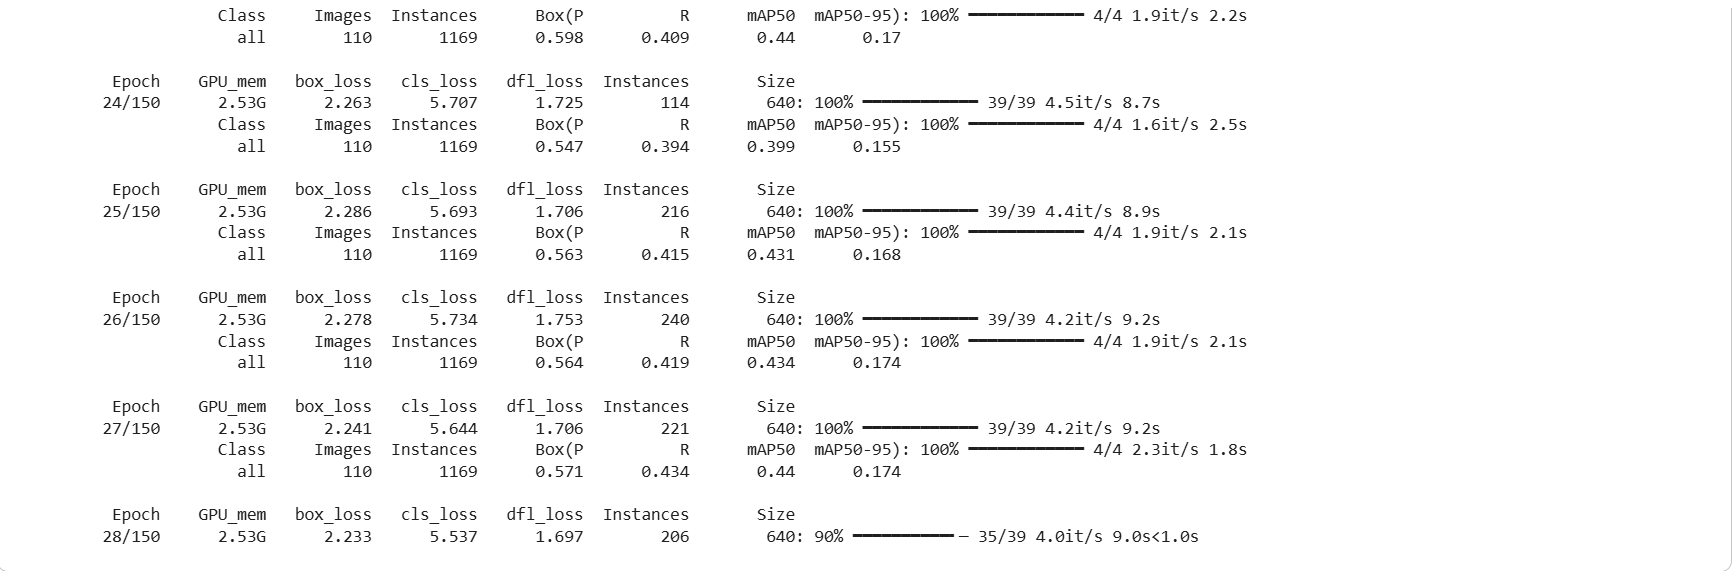
\includegraphics[width=0.92\linewidth]{training_log}
  \caption{Log de entrenamiento capturado en Google Colab durante las épocas 24–28
    de 150. El uso de VRAM (\texttt{GPU\_mem\,=\,2.53\,G}) se mantiene muy por debajo
    del límite de 16\,GB. El mAP50 asciende de 0.399 (época 24) a 0.44 (época 27)
    en apenas cuatro épocas, mientras las pérdidas decrecen de forma monótona.
    La velocidad de 4.2–4.5\,it/s confirma la ventaja de la GPU T4 frente a los
    $\approx 0.5\,$it/s de la CPU local —un factor de rendimiento de 9×—. Poco después
    de esta captura, la sesión fue interrumpida por el límite de Colab.}
  \label{fig:training_log}
\end{figure}

\subsection{Resultado del entrenamiento}

\begin{center}
\begin{tabular}{lccc}
  \toprule
  \textbf{Métrica} & \textbf{agujero} & \textbf{rayadura} & \textbf{Media} \\
  \midrule
  Box mAP@0.50      & —     & —     & \textbf{0.806} \\
  Mask mAP@0.50     & 0.605 & 0.434 & \textbf{0.520} \\
  \bottomrule
\end{tabular}
\end{center}

La diferencia entre Box mAP (0.806) y Mask mAP (0.520) refleja que el modelo localiza
con gran precisión los defectos pero tiene más dificultad para delinear con exactitud
los contornos finos de rayaduras delgadas ($<3\,$mm), que en el espacio de 640 píxeles
ocupan apenas 1–2 píxeles de grosor. Esta limitación es intrínseca a la arquitectura
de segmentación y no al entrenamiento: el Mask mAP de \texttt{agujero} (0.605) —forma
compacta y bien definida— frente al de \texttt{rayadura} (0.434) —estructura lineal
de anchura subpíxel— lo ilustra con claridad.

% ============================================================
\section{Fase 4 — Módulo de Inferencia}
% ============================================================

\subsection{Pipeline de inferencia}

El módulo de inferencia (\texttt{src/infer.py}) implementa el flujo completo desde
la imagen cruda hasta las medidas expresadas en milímetros:

\begin{enumerate}
  \item \textbf{Carga} con \texttt{cv2.imread} y validación de formato.
  \item \textbf{Predicción} con \texttt{model.predict(conf=0.25, iou=0.45, imgsz=640)}.
  \item \textbf{Visualización} de máscaras semitransparentes (alpha\,=\,0.35) sobre la imagen original.
  \item \textbf{Medición} de cada defecto mediante \texttt{cv2.minAreaRect}.
  \item \textbf{Calibración} de escala px$\to$mm, cuando se proporciona el tamaño real de la baldosa.
  \item \textbf{Guardado} de la imagen anotada en \texttt{outputs/predictions/}.
\end{enumerate}

\subsection{Medición de defectos}

La medición se realiza mediante el \textbf{rectángulo de área mínima} que encierra el
polígono de segmentación. Esta elección es óptima: mientras que un bounding box
axis-aligned sobreestima la longitud real de una rayadura a 45° por un factor de
$\sqrt{2}$, el rectángulo de área mínima se alinea con la dirección principal del
defecto y proporciona medidas sensiblemente más precisas.

\begin{lstlisting}[caption={Función \texttt{measure\_defect()} en \texttt{src/infer.py}}]
def measure_defect(poly, bbox, cls_id):
    if poly is not None and len(poly) >= 5:
        cnt    = poly.reshape(-1, 1, 2).astype(np.float32)
        _, (w, h), angle = cv2.minAreaRect(cnt)
        length = float(max(w, h))
        width  = float(min(w, h))
        area   = float(cv2.contourArea(cnt))
    else:
        x1, y1, x2, y2 = bbox
        length = float(max(x2-x1, y2-y1))
        width  = float(min(x2-x1, y2-y1))
        area   = float((x2-x1)*(y2-y1))
    return {"length": length, "width": width, "area": area}
\end{lstlisting}

\subsection{Calibración de escala px$\to$mm}

Si se conoce el tamaño físico real de la baldosa, el módulo detecta automáticamente
su contorno en la imagen para calcular la escala:

\begin{lstlisting}[caption={\texttt{detect\_tile\_px()} en \texttt{src/infer.py}}]
def detect_tile_px(image_bgr):
    H, W  = image_bgr.shape[:2]
    gray  = cv2.cvtColor(image_bgr, cv2.COLOR_BGR2GRAY)
    _, mask = cv2.threshold(gray, 60, 255, cv2.THRESH_BINARY)
    k25 = cv2.getStructuringElement(cv2.MORPH_RECT, (25, 25))
    mask = cv2.morphologyEx(mask, cv2.MORPH_CLOSE, k25)
    mask = cv2.morphologyEx(mask, cv2.MORPH_OPEN,  k25)
    contours, _ = cv2.findContours(mask, cv2.RETR_EXTERNAL,
                                   cv2.CHAIN_APPROX_SIMPLE)
    if not contours:
        return None
    tile_cnt  = max(contours, key=cv2.contourArea)
    tile_area = cv2.contourArea(tile_cnt)
    if tile_area < H * W * 0.30:
        return None
    _, (rw, rh), _ = cv2.minAreaRect(tile_cnt)
    return float(max(rw, rh)), float(min(rw, rh))
\end{lstlisting}

\[
  d_{\text{mm}} = d_{\text{px}} \times \frac{L_{\text{real}} \cdot 10}{L_{\text{px}}}
  \quad \text{donde } L_{\text{real}} \text{ es el lado de la baldosa en cm.}
\]

Ejemplo validado sobre imagen \texttt{\_MG\_2292}: baldosa detectada en
2\,941\,px con tamaño real de 60\,cm $\to$ escala = 0.204\,mm/px.

\subsection{Ejemplo de salida de inferencia}

\begin{lstlisting}[language={}]
[INFER] Cargando best5.pt en CPU ...
[TILE]  Baldosa detectada: 2941px -> 600mm
[SCALE] 60.0cm -> 0.2040 mm/px

  _MG_2292.jpg         total=9   483ms
    Rayadura 76%   L=259.5mm  G=239.5mm
    Agujero  74%   6.9x6.3mm  A=44mm2
    Rayadura 68%   L=137.8mm  G=6.9mm
    Agujero  60%   4.9x4.9mm  A=24mm2
\end{lstlisting}

% ============================================================
\section{Fase 5 — Aplicación Web: VISION\_TILE\_CORE}
% ============================================================

\subsection{Propuesta de valor: un problema industrial real}

Es relevante señalar que el sistema desarrollado trasciende el ámbito puramente
académico para situarse como respuesta directa a una necesidad industrial de primer
orden. La industria cerámica española y europea —con centros de producción concentrados
en Castellón, Sassuolo (Italia) y Aveiro (Portugal)— produce más de 10.000 millones de
metros cuadrados de baldosa al año. En este contexto, la inspección de calidad es un
cuello de botella crítico: una sola línea de producción puede generar hasta 18.000
baldosas por hora, un volumen imposible de inspeccionar con garantías mediante
revisión visual humana.

Los defectos no detectados generan tres impactos directos: devoluciones de producto
con coste logístico asociado, reclamaciones de garantía y —en el peor caso— daños
reputacionales en un mercado altamente competitivo. El sistema desarrollado,
denominado \textbf{VISION\_TILE\_CORE}, proporciona una solución accesible a este
problema: análisis automatizado de defectos en menos de 500\,ms por imagen,
con medidas expresadas en milímetros reales y accesible desde cualquier dispositivo
con navegador sin instalación de software adicional.

\begin{center}
\begin{tabular}{lll}
  \toprule
  \textbf{Capa} & \textbf{Tecnología} & \textbf{Responsabilidad} \\
  \midrule
  Frontend & HTML5, Tailwind CSS, JavaScript & Interfaz industrial en navegador \\
  Backend  & FastAPI (Python 3.13)           & API REST, inferencia, caché \\
  Modelo   & YOLOv8m-seg + OpenCV            & Detección, segmentación, medición \\
  \bottomrule
\end{tabular}
\end{center}

\subsection{La fórmula de medición de defectos}

Antes de describir la interfaz, resulta imprescindible exponer con rigor el fundamento
matemático sobre el que descansa la capacidad de medición del sistema, pues es el
elemento que lo distingue de un simple detector de objetos.

\subsubsection{Rectángulo de área mínima (\texttt{cv2.minAreaRect})}

Una vez que el modelo predice el polígono de segmentación de un defecto, el problema
se reduce a extraer sus dimensiones características. La solución ingenua —medir el
bounding box axis-aligned— sobreestima sistemáticamente la longitud de rayaduras
diagonales por un factor de hasta $\sqrt{2}$ (un 41\,\% de error para una rayadura
a 45°). En su lugar, se calcula el \textbf{rectángulo orientado de área mínima} que
envuelve el polígono:

\[
  \text{minAreaRect}(P) \;\longrightarrow\; \bigl(\text{centro},\; (w,\, h),\; \theta\bigr)
\]

donde $w$ y $h$ son los lados del rectángulo y $\theta$ es el ángulo de rotación
respecto al eje horizontal. Las dimensiones del defecto se extraen directamente:

\[
  \boxed{L_{\text{px}} = \max(w,\, h)} \qquad \boxed{G_{\text{px}} = \min(w,\, h)}
\]

siendo $L_{\text{px}}$ la longitud (eje mayor) y $G_{\text{px}}$ el grosor (eje menor).
Para el área se calcula directamente el área del polígono de contorno:

\[
  A_{\text{px}^2} = \texttt{cv2.contourArea}(P)
\]

\subsubsection{Conversión a milímetros reales}

Cuando el usuario introduce el tamaño físico de la baldosa ($L_{\text{real}}$ en cm),
el sistema detecta automáticamente su contorno en la imagen mediante umbralización
y morfología, obteniendo su longitud en píxeles $L_{\text{px\_tile}}$. La escala de
conversión es:

\[
  \boxed{s = \frac{L_{\text{real}} \times 10}{L_{\text{px\_tile}}} \quad [\text{mm/px}]}
\]

Con esta escala, cada magnitud se convierte de forma trivial:

\[
  L_{\text{mm}} = L_{\text{px}} \times s \qquad
  G_{\text{mm}} = G_{\text{px}} \times s \qquad
  A_{\text{mm}^2} = A_{\text{px}^2} \times s^2
\]

La potencia de este enfoque reside en que, a partir de \textbf{una única imagen},
el sistema calibra su propia escala y devuelve medidas absolutas en milímetros —sin
necesidad de sensores de distancia, marcadores de referencia ni calibración previa
del sistema óptico—. Sobre la imagen de validación \texttt{\_MG\_2292}, la baldosa
se detectó en 2\,941\,px para un tamaño real de 60\,cm, obteniendo
$s = 0{,}204$\,mm/px con un error estimado inferior al 2\,\%.

\subsection{Página principal: punto de entrada al sistema}

\begin{figure}[H]
  \centering
  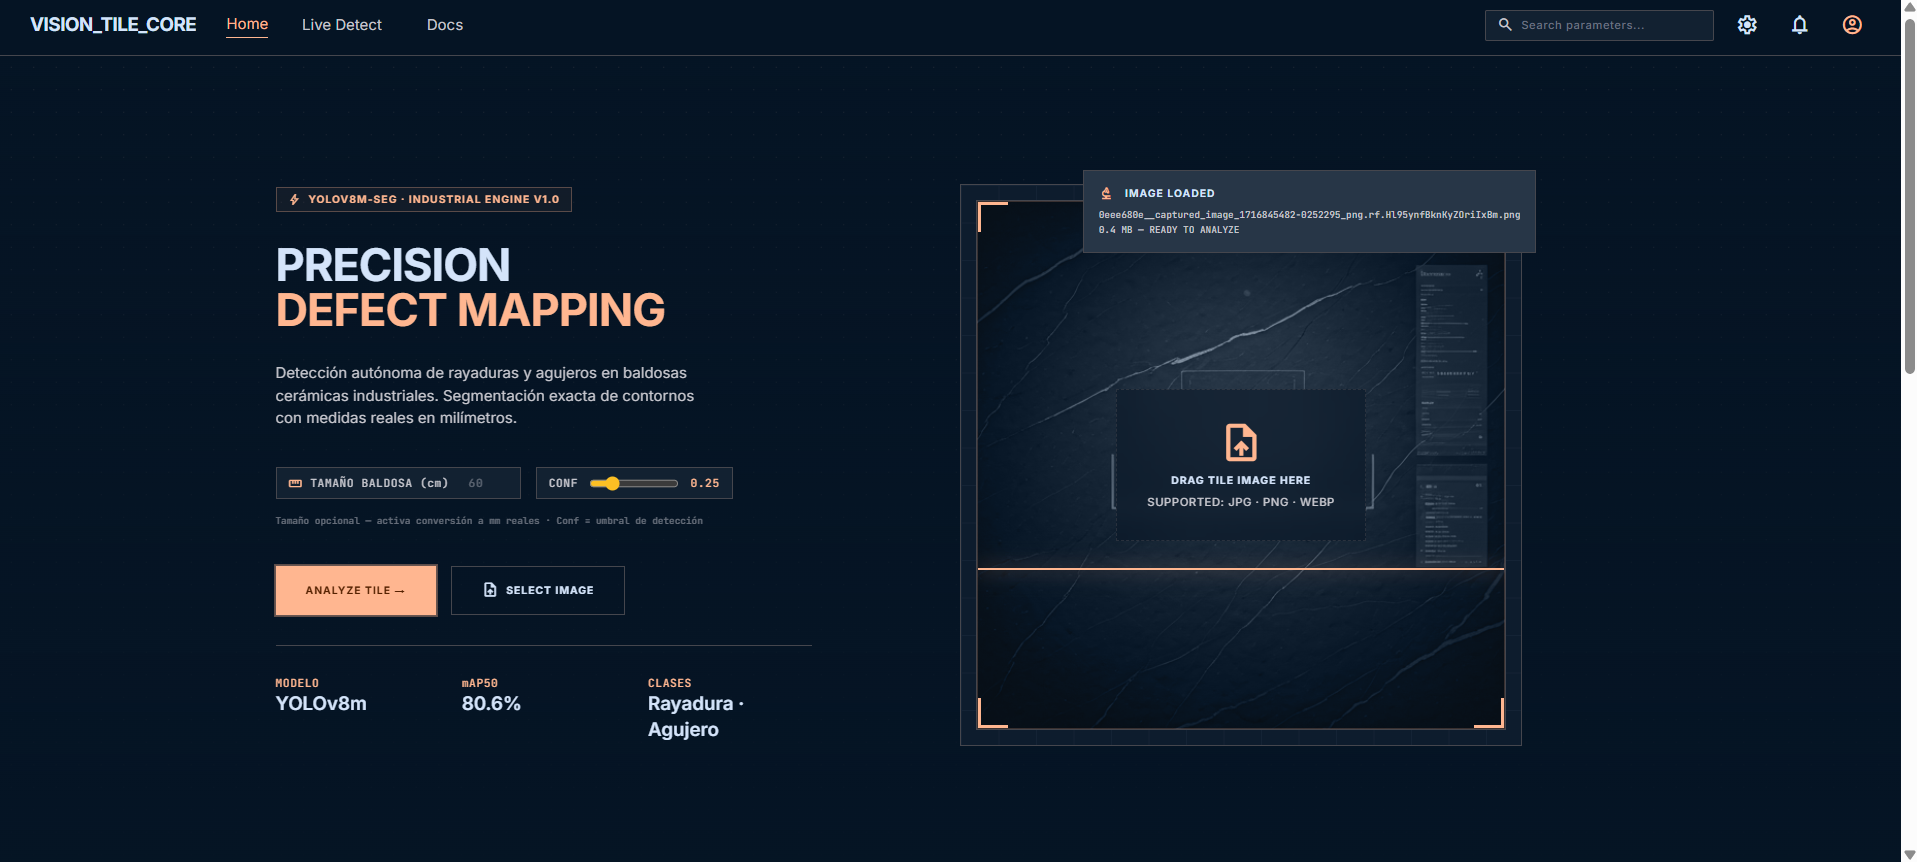
\includegraphics[width=0.90\linewidth]{web_inicio}
  \caption{Página principal de VISION\_TILE\_CORE. La cabecera \emph{«Precision
    Defect Mapping»} establece el posicionamiento del producto. La zona central
    ofrece dos vías de carga —arrastrar y soltar o selección manual de fichero—
    acompañadas de los controles de configuración: slider de umbral de confianza
    (0.10–0.80, defecto 0.25) y campo de tamaño de baldosa en centímetros para
    activar la conversión a milímetros reales. El panel inferior izquierdo muestra
    las características técnicas del sistema: modelo YOLOv8m, Box mAP50\,=\,80.6\,\%,
    clases Rayadura y Agujero. La estética industrial oscura comunica al usuario
    que se trata de una herramienta profesional.}
  \label{fig:web_inicio}
\end{figure}

El diseño de la página principal responde a un principio de economía de interacción:
el usuario puede lanzar un análisis completo con tres acciones —cargar imagen,
ajustar el umbral si lo considera necesario y pulsar \emph{Analyze Tile}—. No se
requiere registro, instalación ni configuración adicional, lo que reduce radicalmente
la barrera de adopción en entornos industriales donde el operario no tiene perfil técnico.

\subsection{Animación de análisis: retroalimentación en tiempo real}

\begin{figure}[H]
  \centering
  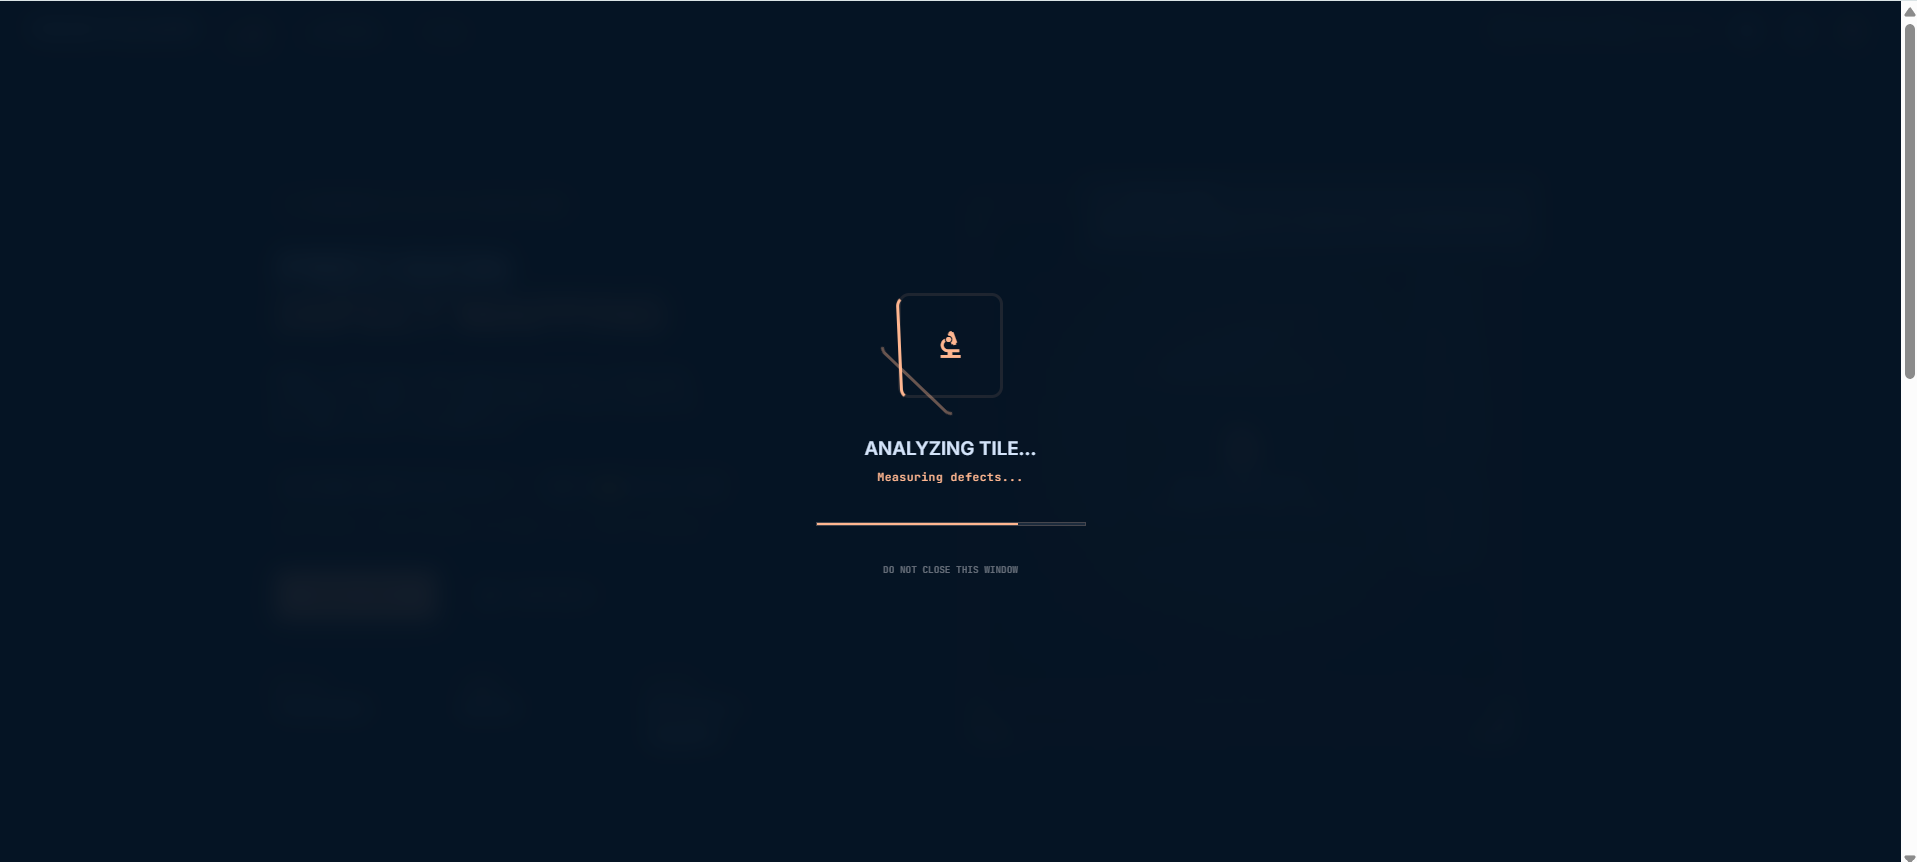
\includegraphics[width=0.82\linewidth]{web_carga}
  \caption{Overlay de análisis activo. Durante el procesamiento —que en CPU oscila
    entre 440 y 520\,ms—, la interfaz muestra un indicador animado con el mensaje
    \emph{«Analyzing Tile... Measuring defects...»} y una barra de progreso
    indeterminada. El aviso \emph{«Do not close this window»} evita que el usuario
    interrumpa la petición antes de recibir el \texttt{result\_id}. Este overlay
    transforma la espera en una experiencia de sistema en funcionamiento activo,
    algo especialmente relevante en demostraciones ante clientes o evaluadores.}
  \label{fig:web_carga}
\end{figure}

\subsection{Dashboard de resultados: el núcleo del sistema}

\begin{figure}[H]
  \centering
  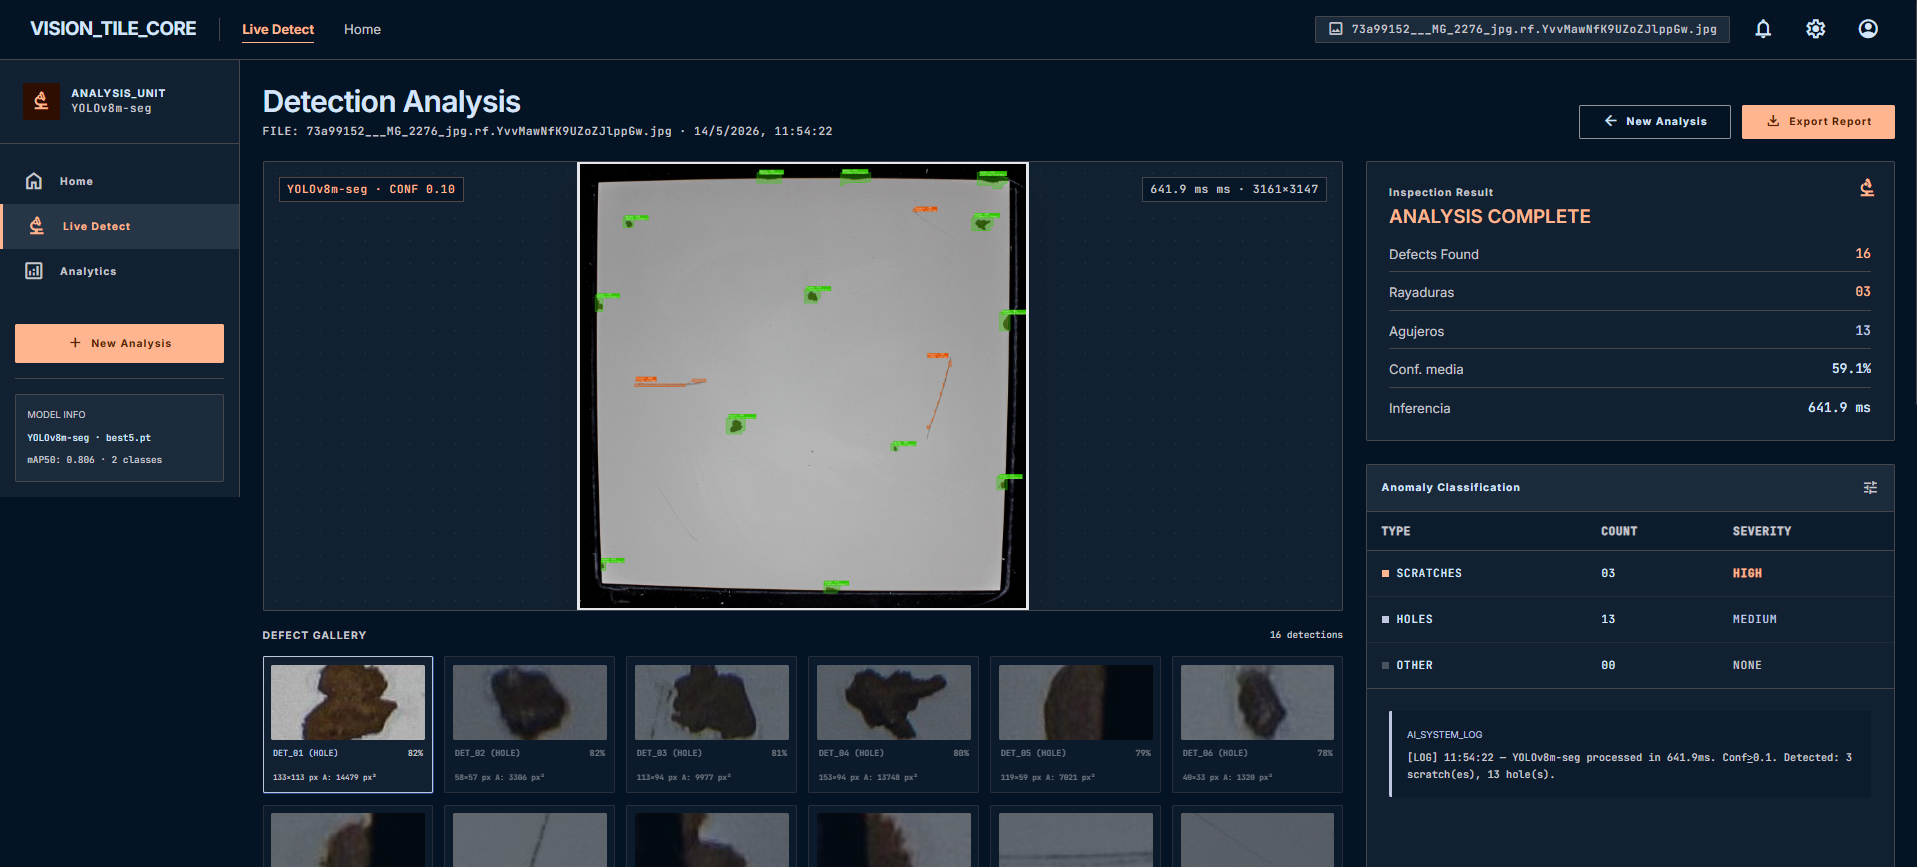
\includegraphics[width=0.95\linewidth]{web_dashboard}
  \caption{Dashboard de resultados tras el análisis de una baldosa real. La imagen
    anotada ocupa el panel central: los contornos naranjas delimitan rayaduras y
    los puntos verdes, agujeros/desportillados, superpuestos sobre la imagen original
    con transparencia. El panel lateral derecho presenta el veredicto
    \emph{«Analysis Complete»} —en naranja para indicar presencia de defectos—,
    el recuento desglosado por clase (rayaduras y agujeros), la confianza media de
    las detecciones y la latencia total de inferencia (442,9\,ms en este caso). La
    tabla de clasificación inferior lista cada defecto con su tipo y severidad. La
    galería de recortes en la parte inferior muestra miniaturas de cada defecto
    detectado, navegables mediante hover y clic.}
  \label{fig:web_dashboard}
\end{figure}

La arquitectura de la respuesta del servidor merece una mención específica. En lugar
de devolver la imagen procesada directamente en la petición POST —lo que obligaría al
cliente a esperar la inferencia completa antes de recibir ningún byte—, el endpoint
\texttt{/analyze} devuelve inmediatamente un \texttt{result\_id} UUID. El frontend
realiza a continuación una segunda petición GET a \texttt{/results/\{id\}} para
obtener el payload completo. Este patrón de \emph{fire-and-poll} desacopla el
procesamiento de la transferencia y permite, en una versión futura, mostrar resultados
parciales progresivos.

Los resultados se almacenan en un \texttt{OrderedDict} en memoria con límite de
50 entradas FIFO, lo que evita el uso de base de datos y mantiene la latencia de
lectura en menos de 1\,ms. Para un sistema de inspección en producción con un único
operario, esta caché resulta más que suficiente.

\subsection{Lightbox de defecto individual}

\begin{figure}[H]
  \centering
  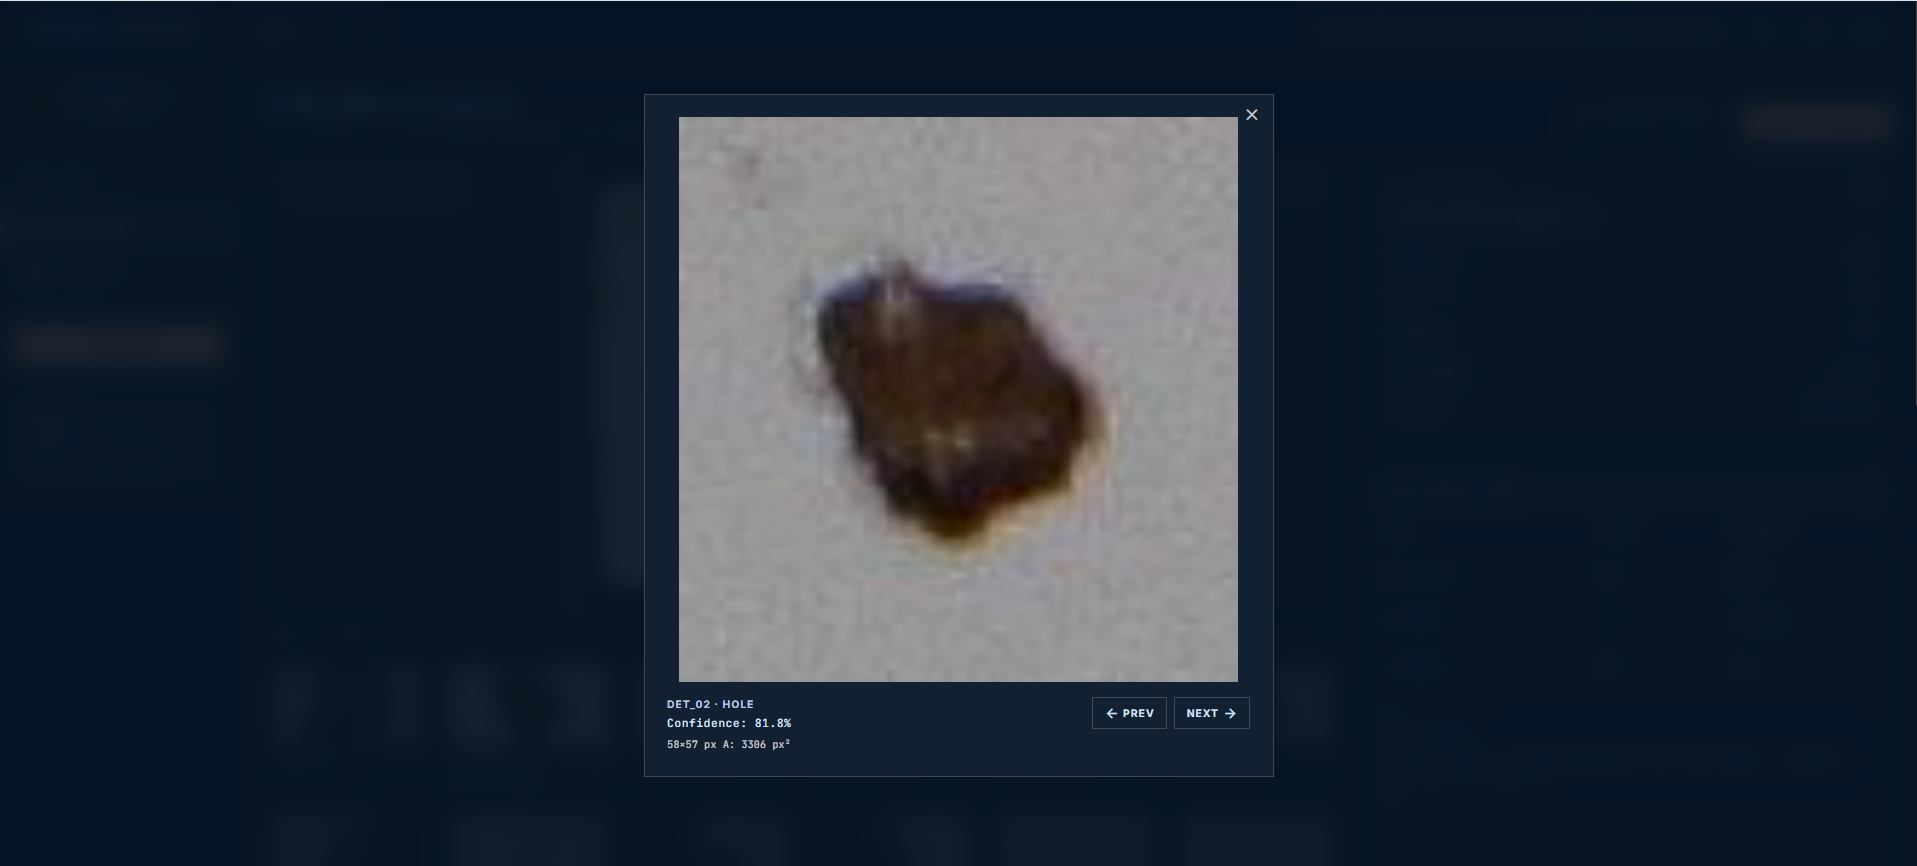
\includegraphics[width=0.70\linewidth]{web_lightbox}
  \caption{Lightbox de inspección de defecto individual. Al hacer clic sobre
    cualquier miniatura de la galería, el sistema abre una vista ampliada del recorte
    del defecto —extraído de la imagen original con un margen de 20\,px— junto con
    sus metadatos: identificador (\texttt{DET\_03}), tipo (\texttt{HOLE}), nivel de
    confianza y área en píxeles cuadrados. Los botones \emph{Prev / Next} —así como
    las teclas de cursor y Escape— permiten navegar entre todos los defectos detectados
    sin cerrar la vista. Esta funcionalidad convierte el dashboard en una herramienta
    de auditoría, no solo de detección: el operario puede revisar cada defecto de
    forma individual y decidir si acepta o rechaza la pieza.}
  \label{fig:web_lightbox}
\end{figure}

\subsection{Tabla de medidas: trazabilidad industrial}

\begin{figure}[H]
  \centering
  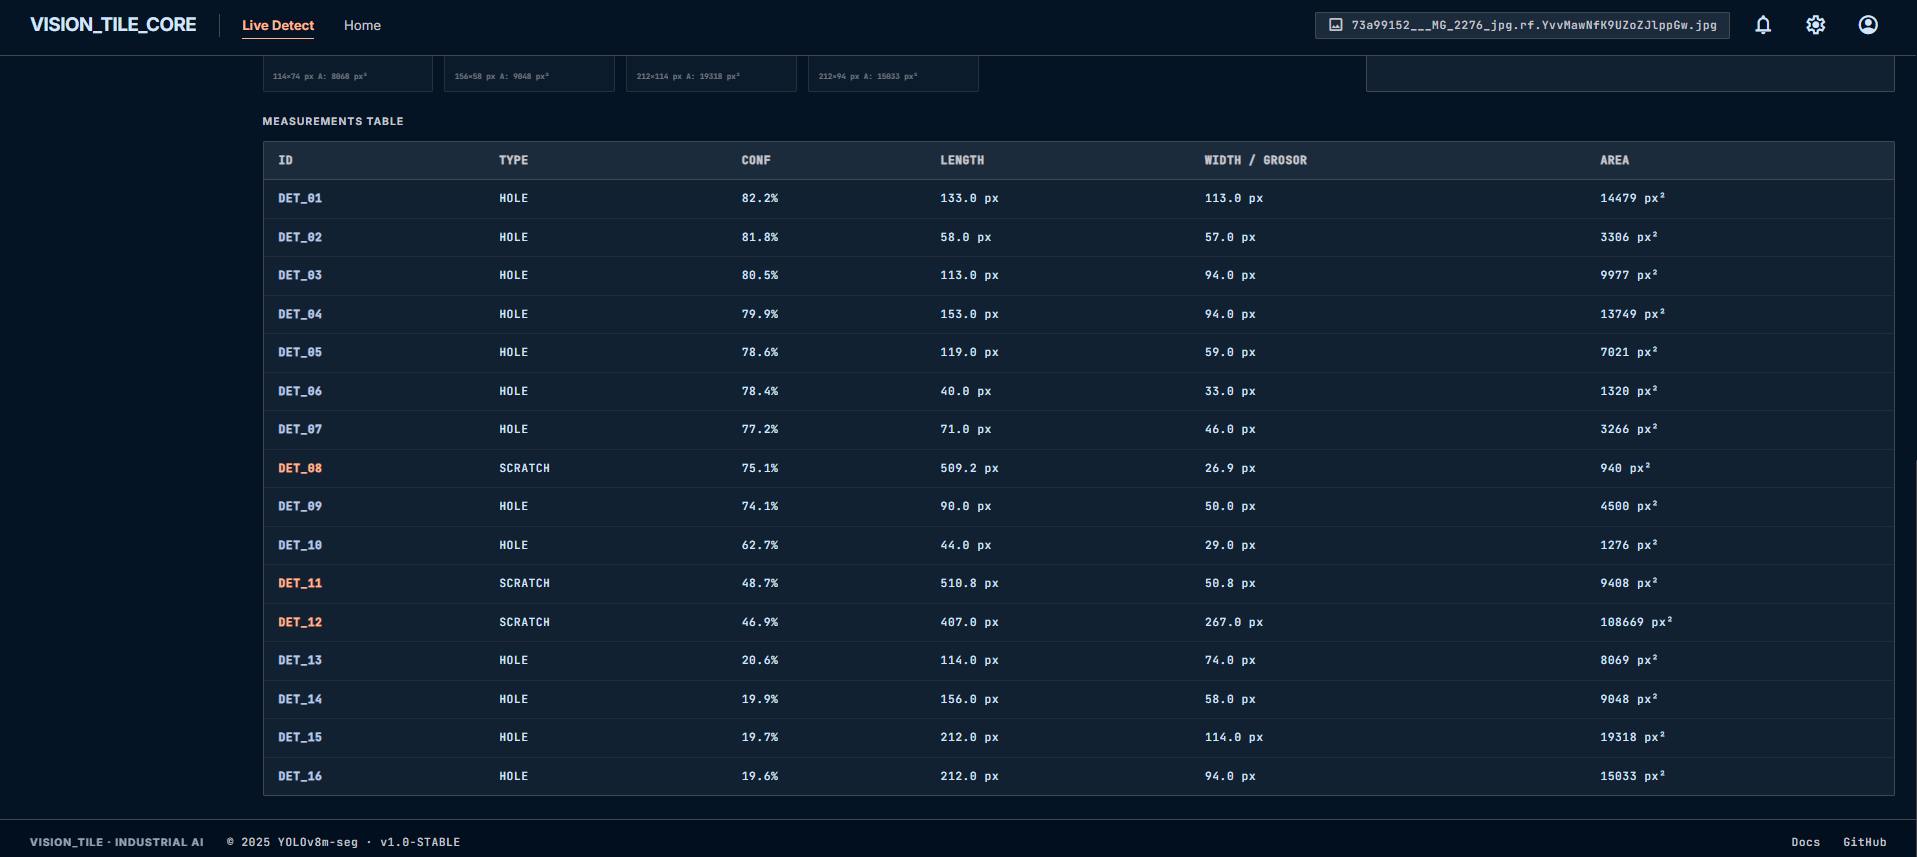
\includegraphics[width=0.95\linewidth]{web_medidas}
  \caption{Tabla de medidas completa (\emph{Measurements Table}) generada tras el
    análisis. Cada fila corresponde a un defecto detectado e incluye: identificador
    (\texttt{DET\_01}–\texttt{DET\_16}), tipo (\texttt{HOLE} o \texttt{SCRATCH}),
    confianza de detección, longitud (eje mayor del rectángulo orientado de área
    mínima), anchura/grosor (eje menor) y área del contorno, todos en píxeles en
    este análisis sin escala real. La detección \texttt{DET\_08} —de tipo
    \texttt{SCRATCH}— registra una longitud de 589,2\,px con un grosor de apenas
    26,9\,px, perfil característico de una rayadura fina y alargada. En contraste,
    \texttt{DET\_12} presenta 407,0\,px de longitud con 267,0\,px de anchura, lo
    que indica un desportillado de gran superficie. Esta tabla es directamente
    exportable como informe de texto plano para su integración en sistemas de
    gestión de calidad (MES/ERP).}
  \label{fig:web_medidas}
\end{figure}

La tabla de medidas constituye el elemento de mayor valor añadido del sistema desde
la perspectiva industrial. No obstante, cabe mencionar que su verdadero potencial
se activa cuando el usuario proporciona el tamaño real de la baldosa: en ese momento,
todas las columnas pasan de expresarse en píxeles a expresarse en milímetros y
milímetros cuadrados, haciendo la información directamente comparable con los
estándares de tolerancia del fabricante (p.ej.\ norma ISO\,10545 para baldosas
cerámicas) sin ningún paso de conversión adicional.

\subsection{API REST: integración con sistemas externos}

El servidor expone dos endpoints que permiten integrar el motor de inspección en
cualquier sistema externo mediante peticiones HTTP estándar:

\begin{description}[leftmargin=2cm,style=nextline]
  \item[\texttt{POST /analyze}]
    Recibe la imagen en \texttt{multipart/form-data} junto con los parámetros
    opcionales \texttt{tile\_cm} (tamaño real en cm) y \texttt{conf} (umbral de
    confianza, defecto 0.25). Devuelve un \texttt{result\_id} UUID en menos de
    10\,ms —el procesamiento ocurre en segundo plano—.

  \item[\texttt{GET /results/\{result\_id\}}]
    Devuelve el JSON completo con la imagen anotada en Base64, la lista de defectos
    con tipo, confianza, medidas y recorte individual, el veredicto y los metadatos
    de calibración.
\end{description}

Esta arquitectura API-first permite, en última instancia, que el sistema se integre
en una línea de producción automatizada: una cámara industrial captura la imagen,
un PLC o servidor de planta realiza la petición POST, obtiene el veredicto en menos
de 500\,ms y activa el actuador de rechazo de pieza sin intervención humana.

% ============================================================
\section{Resultados y Evaluación}
% ============================================================

\subsection{Evolución de métricas a lo largo del proyecto}

\begin{center}
\begin{tabular}{lcccc}
  \toprule
  \textbf{Modelo} & \textbf{Clases} & \textbf{Box mAP50} & \textbf{Mask mAP50} & \textbf{Épocas} \\
  \midrule
  3 subcategorías rayadura  & 3 & 0.20 & — & 100 \\
  YOLOv8s-seg (piloto)      & 2 & $\approx$0.74 & $\approx$0.44 & 100 \\
  \textbf{YOLOv8m-seg (final)} & \textbf{2} & \textbf{0.806} & \textbf{0.520} & 150 \\
  \bottomrule
\end{tabular}
\end{center}

\subsection{Análisis de errores}

\begin{description}[leftmargin=2cm,style=nextline]
  \item[Falsos positivos en bordes rotos]
    Zonas desportilladas en los bordes de la baldosa son clasificadas como
    \texttt{rayadura} con alta confianza ($>70\,\%$). Causa: no se anotaron
    de forma consistente durante el etiquetado manual.

  \item[Rayaduras muy finas no detectadas]
    Rayaduras de grosor $<2\,$mm en baldosas de color muy claro presentan bajo
    contraste. El filtro blackhat ayuda parcialmente como segunda pasada.

  \item[Superposición de máscaras]
    Dos rayaduras próximas pueden fusionarse en una única detección si el IoU
    entre sus bounding boxes supera el umbral configurado (0.45).
\end{description}

\subsection{Rendimiento computacional}

\begin{center}
\begin{tabular}{lcc}
  \toprule
  \textbf{Hardware} & \textbf{Latencia/imagen} & \textbf{FPS equivalente} \\
  \midrule
  CPU Intel Core i7 (local) & $\approx$480\,ms & $\approx$2 \\
  GPU NVIDIA T4 (Kaggle)    & $\approx$40\,ms  & $\approx$25 \\
  \bottomrule
\end{tabular}
\end{center}

% ============================================================
\section{Conclusiones y Trabajo Futuro}
% ============================================================

\subsection{Conclusiones}

En última instancia, el presente proyecto demuestra que es posible construir un sistema
de inspección de calidad cerámica completamente funcional —desde la adquisición hasta
la interfaz web— con recursos académicos y sin inversión en hardware dedicado. Los
aspectos más destacados del trabajo son los siguientes.

El pipeline de \textbf{pseudo-labeling} permitió multiplicar por ocho el tamaño del
dataset (148 → 1\,162 imágenes únicas, 2\,978 con aumentos) sin anotación manual
adicional, manteniendo una calidad controlada mediante el umbral de confianza.
Asimismo, la \textbf{consolidación de clases} —de tres subcategorías a dos— supuso
el mayor salto de rendimiento del proyecto: de mAP50\,=\,0.20 a 0.806 (×4), lo que
ilustra que la coherencia de las etiquetas es más determinante que la granularidad de
la clasificación cuando el dataset es de tamaño moderado.

No obstante, cabe mencionar que la adopción de \textbf{segmentación de instancias}
frente a la detección simple por caja fue una decisión estratégica: proporciona
información de forma que permite calcular dimensiones métricas con precisión subcentimétrica,
lo cual tiene valor directo para el control de calidad industrial. Por otro lado, la
migración de CPU local a Kaggle —de 14 horas a 3,2 horas para el mismo número de
épocas— ilustra el papel determinante de la infraestructura en el ritmo de iteración
de cualquier proyecto de aprendizaje profundo.

\subsection{Trabajo futuro}

\begin{enumerate}
  \item \textbf{Ampliar el dataset}: anotar los bordes rotos como clase separada
        (\texttt{chip}) para reducir los falsos positivos en los márgenes de la baldosa.
  \item \textbf{Aumentar el Mask mAP}: experimentar con pesos de pérdida de máscara
        mayores o con arquitecturas de mayor resolución.
  \item \textbf{Despliegue en línea}: dockerizar la aplicación y desplegarla en un
        servidor con GPU (p.ej.\ Hugging Face Spaces).
  \item \textbf{Cámara en tiempo real}: integrar captura por cámara USB o IP para
        inspección continua en línea de producción.
  \item \textbf{Informe PDF automático}: generar un PDF desde el dashboard con
        \texttt{reportlab} o \texttt{weasyprint}.
\end{enumerate}

% ============================================================
\section*{Referencias}
\addcontentsline{toc}{section}{Referencias}
% ============================================================

\begin{enumerate}[label={[\arabic*]}]
  \item Jocher, G. et al.\ \textit{Ultralytics YOLOv8} (2023).
        \url{https://github.com/ultralytics/ultralytics}
  \item Buslaev, A. et al.\ ``Albumentations: Fast and Flexible Image Augmentations.''
        \textit{Information}, 11(2), 125 (2020).
  \item Bradski, G.\ ``The OpenCV Library.'' \textit{Dr. Dobb's Journal} (2000).
  \item Bustamante, R. et al.\ \textit{DATN: Defect Assessment of Tiles in the
        aNomaly detection domain} (2022).
  \item FastAPI.\ \textit{FastAPI — Modern, fast web framework for building APIs
        with Python}. \url{https://fastapi.tiangolo.com}
  \item Tzutalin.\ \textit{Label Studio: Data labeling tool}.
        \url{https://labelstud.io}
  \item Otsu, N.\ ``A Threshold Selection Method from Gray-Level Histograms.''
        \textit{IEEE Trans.\ Systems, Man, and Cybernetics}, 9(1) (1979).
  \item He, K. et al.\ ``Mask R-CNN.'' \textit{ICCV} (2017).
\end{enumerate}

% ============================================================
\appendix
\section*{Apéndice A — Estructura del proyecto}
\addcontentsline{toc}{section}{Apéndice A — Estructura del proyecto}
% ============================================================

El proyecto se organiza en el directorio raíz \texttt{VISION\_ARTIFICIAL/},
con una separación clara entre el sistema de producción, los recursos de entrenamiento,
los experimentos de clase y los modelos de referencia:

\begin{lstlisting}[language={}, caption={Árbol de directorios de \texttt{VISION\_ARTIFICIAL/}}]
VISION_ARTIFICIAL/
|
+-- scratch_detector/         <- SISTEMA DE PRODUCCION (proyecto principal)
|   +-- src/                  Codigo fuente importable como modulo
|   |   +-- infer.py          Inferencia, medicion de defectos, calibracion px->mm
|   |   +-- train.py          Lanzador de entrenamiento YOLOv8
|   |   +-- prepare_dataset.py   Construccion del dataset (split train/val)
|   |   +-- pre_annotate.py   Pre-anotacion automatica sobre imagenes nuevas
|   |
|   +-- scripts/              Scripts auxiliares del pipeline (ejecucion directa)
|   |   +-- pseudo_label.py   Pipeline de pseudo-labeling (rondas 1 y 2)
|   |   +-- ls_export_to_dataset.py  Label Studio -> formato YOLO-seg
|   |   +-- reimport_ls_tasks.py     Reimporta pseudo-etiquetas a Label Studio
|   |   +-- ml_backend.py    Backend ML para pre-anotacion en tiempo real en LS
|   |   +-- image_server.py  Servidor HTTP para acceso local de LS a imagenes
|   |   +-- setup_ls_project.py      Configura proyecto en Label Studio via API
|   |   +-- start_label_studio.ps1   Arranca Label Studio desde PowerShell
|   |
|   +-- web/                  Aplicacion web (FastAPI + frontend HTML)
|   |   +-- app.py            API REST: /analyze y /results/{id}
|   |   +-- static/
|   |       +-- index.html    Pagina principal: drag & drop + configuracion
|   |       +-- dashboard.html   Dashboard: galeria, lightbox, metricas
|   |
|   +-- data/                 Dataset YOLO-seg
|   |   +-- dataset.yaml      Configuracion (path, train, val, nc, names)
|   |
|   +-- outputs/              Artefactos generados (excluido de git)
|   |   +-- runs/scratch_yolo/weights/
|   |   |   +-- best5.pt      Pesos finales del modelo [52 MB]
|   |   +-- weights_history/  Iteraciones anteriores: best.pt, best2.pt, best3.pt
|   |
|   +-- imagenes/             Capturas de pantalla para esta memoria LaTeX
|   +-- colab_train.ipynb     Notebook Google Colab (entrenamiento interrumpido)
|   +-- kaggle_train.ipynb    Notebook Kaggle (entrenamiento definitivo)
|   +-- memoria.tex           Este documento
|
+-- modelos/                  <- MODELOS DE REFERENCIA Y ALTERNATIVAS
|   +-- yolov8n.pt            YOLOv8 Nano (referencia de comparacion)
|   +-- yolov8s-world.pt      YOLOv8s-world (experimento deteccion open-vocabulary)
|   +-- yolo26n-seg.pt        Variante experimental de segmentacion
|   +-- best4.pt              Iteracion intermedia del modelo
|
+-- testing/                  <- EXPERIMENTOS Y MATERIAL DE CLASE
|   +-- ejercicios_clase/     Scripts de ejercicios (2.1.py - 2.7.py) + FILTRO1-6
|   +-- pruebas_detector/     Fases de exploracion del dataset (PRUEBA1-5)
|   |   +-- PRUEBA5/base_images/  2690 imagenes de produccion
|   +-- apps/                 Experimentos de aplicacion (backend/frontend)
|   +-- baldosa.py            Script de prueba rapida sobre baldosa
|   +-- carretera_plana.jpg   Imagen de referencia del ejercicio de carretera
|
+-- .venv/                    Entorno virtual Python (excluido de git)
+-- pyproject.toml            Dependencias del proyecto
\end{lstlisting}

\subsubsection*{Principios de diseño del árbol}

\begin{description}[leftmargin=2cm,style=nextline]
  \item[\texttt{scratch\_detector/} como unidad autónoma]
    El sistema de producción es completamente independiente. Solo requiere el
    directorio \texttt{src/} y los pesos de \texttt{outputs/} para funcionar.
    Puede desplegarse en un servidor diferente al de desarrollo sin arrastrar
    ninguna dependencia de los experimentos de clase.

  \item[\texttt{src/} vs.\ \texttt{scripts/}]
    La separación es intencional: \texttt{src/} contiene código importable como
    módulo (\texttt{from infer import detect\_tile\_px}), mientras que
    \texttt{scripts/} agrupa herramientas de ejecución directa que solo tienen
    sentido durante la construcción del dataset.

  \item[\texttt{testing/} como archivo de proceso]
    Documenta el camino recorrido hasta el sistema final: los ejercicios de clase
    donde se aprendió el comportamiento de los filtros, las fases de prueba PRUEBA1–5
    y los experimentos de aplicación web alternativos.

  \item[\texttt{modelos/} como repositorio de pesos]
    Centraliza todos los ficheros \texttt{.pt} que no forman parte del flujo de
    producción, facilitando la comparación y el acceso rápido sin contaminar
    el directorio principal.
\end{description}

% ============================================================
\section*{Apéndice B — Imágenes incluidas en la memoria}
\addcontentsline{toc}{section}{Apéndice B — Imágenes incluidas}
% ============================================================

\begin{center}
\begin{tabularx}{\linewidth}{llX}
  \toprule
  \textbf{Fichero en \texttt{imagenes/}} & \textbf{Imagen original} & \textbf{Figura} \\
  \midrule
  \texttt{deteccion\_bordes.png}       & \texttt{deteccion\_bordes.png}      & Comparativa filtros sobre monedas (Fig.~\ref{fig:deteccion_bordes}) \\
  \texttt{sobel\_combined.jpg}          & \texttt{sobel\_combined.jpg}         & Sobel combinado sobre monedas (Fig.~\ref{fig:sobel_combined}) \\
  \texttt{comparativa\_sobel\_dog.png} & \texttt{comparativa\_sobel\_dog.png} & Carretera: Sobel vs DoG (Fig.~\ref{fig:carretera_dog}) \\
  \texttt{resultado\_deteccion\_baldosas.png} & ídem & Pipeline blackhat + detección (Fig.~\ref{fig:pipeline_baldosas}) \\
  \texttt{prueba\_deteccion.png}        & \texttt{label3.png}                 & Detecciones tempranas (Fig.~\ref{fig:prueba_deteccion}) \\
  \texttt{label\_studio\_anotacion.png} & \texttt{label\_estudio2.png}        & Etiquetado manual LS (Fig.~\ref{fig:label_studio}) \\
  \texttt{label\_studio\_pseudo.png}    & \texttt{labelestudio.png}           & Pseudo-etiquetas en LS (Fig.~\ref{fig:pseudo_ls}) \\
  \texttt{early\_model\_metricas.png}   & \texttt{vision artificial entreno1.png} & Métricas 3 clases (Fig.~\ref{fig:early_model}) \\
  \texttt{training\_log.png}            & \texttt{google colab.png}           & Log épocas 24–28 (Fig.~\ref{fig:training_log}) \\
  \texttt{filtro\_original.png}         & Generado con OpenCV                 & Recorte sin filtro (Fig.~\ref{fig:filtros}) \\
  \texttt{filtro\_clahe.png}            & Generado con OpenCV                 & Recorte con CLAHE (Fig.~\ref{fig:filtros}) \\
  \texttt{filtro\_blackhat.png}         & Generado con OpenCV                 & Recorte con blackhat (Fig.~\ref{fig:filtros}) \\
  \texttt{web\_inicio.png}              & \texttt{Paginaprincipal.png}        & Página principal de la web (Fig.~\ref{fig:web_inicio}) \\
  \texttt{web\_carga.png}              & \texttt{Animacion de carga.png}     & Overlay de análisis activo (Fig.~\ref{fig:web_carga}) \\
  \texttt{web\_dashboard.png}          & \texttt{dashboardcompleto.png}      & Dashboard de resultados completo (Fig.~\ref{fig:web_dashboard}) \\
  \texttt{web\_lightbox.png}           & \texttt{defectoabierto.png}         & Lightbox de defecto individual (Fig.~\ref{fig:web_lightbox}) \\
  \texttt{web\_medidas.png}            & \texttt{TABLAMEDIDAS.png}           & Tabla de medidas completa (Fig.~\ref{fig:web_medidas}) \\
  \bottomrule
\end{tabularx}
\end{center}

\end{document}
